\documentclass[table]{beamer}
\usepackage[utf8]{inputenc}
\usepackage{xcolor}
\usepackage{tcolorbox}
\usepackage{adjustbox}
\usepackage{multicol}
\usepackage{multirow}
\usepackage{eurosym}
\usepackage{amsmath}
\usepackage{ragged2e}
\usepackage[scaled]{helvet}
\usepackage{tikz}
\usepackage{eurosym}
\usetikzlibrary{spy,shapes,arrows,positioning,decorations.pathreplacing,matrix,calligraphy,calc}

\tikzset{hide on/.code={\only<#1>{\color{white}}}}
\definecolor{dark_green}{rgb}{0.0, 0.5, 0.0}

\pgfdeclarelayer{bg}    % declare background layer
\pgfsetlayers{bg,main}  % set the order of the layers (main is the standard layer)

\apptocmd{\frame}{}{\justifying}{}

\definecolor{iscal_color}{HTML}{641242} % ISCAL

\setbeamertemplate{footline}{
	\hspace{0.05\textwidth}
	\raisebox{3ex}{\insertshortauthor{}}\hfill
	\raisebox{3ex}{\insertframenumber{}/\inserttotalframenumber} \hfill
	{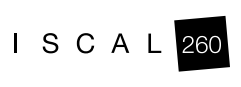
\includegraphics[height=0.08\textheight]{../visual material/logo.png}}
	\hspace{0.05\textwidth}
}

\tikzset{
  invisible/.style={opacity=0},
  visible on/.style={alt={#1{}{invisible}}},
  alt/.code args={<#1>#2#3}{%
    \alt<#1>{\pgfkeysalso{#2}}{\pgfkeysalso{#3}} % \pgfkeysalso doesn't change the path
  },
}

\title{Microeconomia}
\subtitle{Capitulo 3 : Teoria do Produtor}
\author[]{}
\institute[ISCAL]{
\includegraphics[height=0.10\textheight]{../visual material/logo_eng_full.png}}
\date{}

\setbeamertemplate{navigation symbols}{}

\setbeamercolor{title}{fg = iscal_color}
\setbeamercolor{subtitle}{fg = iscal_color}
\setbeamercolor{frametitle}{fg = white, bg = iscal_color}

\hypersetup{linkcolor=iscal_color, colorlinks=true}

\AtBeginSection{\frame{\sectionpage}}
\renewcommand{\sectionname}{Parte}

\begin{document}

{
\setbeamertemplate{footline}{}
\begin{frame}
	\maketitle
\end{frame}
}

\begin{frame}{Conte\'udos}
  \tableofcontents
\end{frame}

\section{Geometria dos custos}
\input{lecture 13}
\section{Solu\c c\~ao anal\'itica do problema do produtor}
\begin{frame}
	\frametitle{Em Geral...}
	\begin{center}
		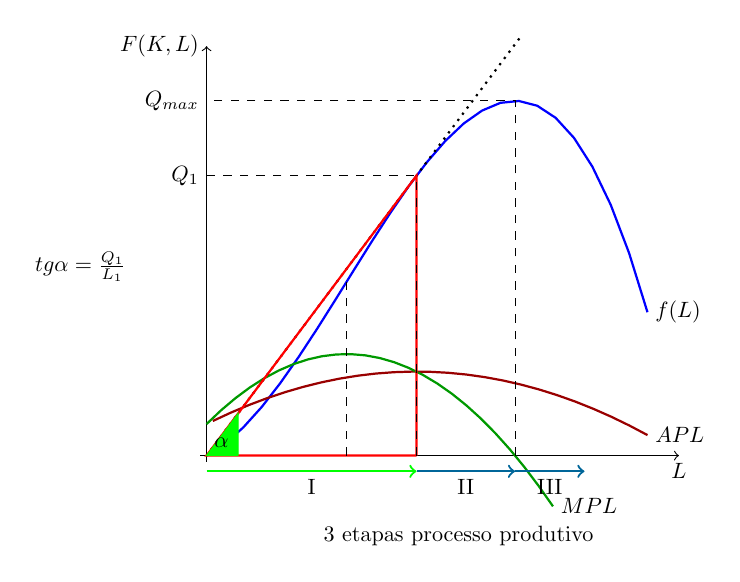
\begin{tikzpicture}[
			scale = 0.8,
			every node/.style = {scale = 0.8},
			declare function = {
				f(\x)=1*(\x/2)+2*(\x/2)^2-0.6*(\x/2)^3;
				apl(\x) = f(\x)/\x;
				mpl(\x) = 1/2+\x-0.225*\x^2;
				tgt(\x) = 0 + apl(10/3)*\x;
			}
			]

			\draw[->] (-0.1,0) -- (7.5,0) node[below]{$L$};
			\draw[->] (0,-0.1) -- (0,6.5) node[left]{$F(K,L)$};

			\draw[blue,thick,domain = 0:7,variable=\x,samples=25] plot (\x,{f(\x)});
			\draw[red!60!black,thick,domain = 0.1:7,variable=\x,samples=25] plot (\x,{apl(\x)});
			\draw[green!60!black,thick,domain = 0:5.5,variable=\x,samples=25] plot (\x,{mpl(\x)});

			\onslide<2->{
				\draw[dotted,thick,domain=0:5,variable=\x] plot (\x,{tgt(\x)});
			}

			\onslide<3-5>{
				\draw[red,thick] ({10/3},0) -- ({10/3},{f(10/3)}) -- (0,0) -- ({10/3},0);
			}

			\onslide<4-5>{
				\draw[green,fill] ({1.5/3},0) -- ({1.5/3},{tgt(1.5/3)}) -- (0,0) -- ({1.5/3},0);
				\draw(0,0) node[above right]{$\alpha$};
			}

			\only<5>{
				\draw(-2,3) node[]{\(tg\alpha=\frac{Q_1}{L_1}\)};
			}

			\onslide<1-5>{
				\draw(7,{f(7)}) node[right]{$f(L)$};
				\draw(7,{apl(7)}) node[right]{$APL$};
				\draw(5.5,{mpl(5.5)}) node[right]{$MPL$};
			}

			\draw[dashed] ({20/9},0) --({20/9},{f(20/9)});
			\draw[dashed] (4.89813,0) -- (4.89813,{f(4.89813)}) -- (0,{f(4.89813)})node[left]{$Q_{max}$};
			\draw[dashed] ({10/3},0) -- ({10/3},{f(10/3)}) -- (0,{f(10/3)})node[left]{$Q_1$};

			\onslide<6->{
				\draw[->,thick,green] (0,-0.25) -- ({10/3},-0.25) node[black,midway,yshift=-0.25cm]{I};
				\draw[->,thick,blue!60!green] ({10/3},-0.25) -- (4.89813,-0.25)node[black,midway,yshift=-0.25cm]{II};
				\draw[->,thick,blue!60!green] (4.89813,-0.25) -- (6,-0.25)node[black,midway,yshift=-0.25cm]{III};

				\draw(4,-1) node[below]{3 etapas processo produtivo};
			}
		\end{tikzpicture}
	\end{center}

	\onslide<6->{Etapa II: Zona econ\'omica de explora\c c\~ao, entre $Q_1$ e $Q_{max}$ \'e que estar\~ao as escolhas \'otimas de produ\c c\~ao para o produtor.}
\end{frame}

\begin{frame}
	\frametitle{Fun\c c\~ao de Produ\c c\~ao}
	As fun\c c\~oes de produ\c c\~ao podem ser representadas por express\~oes anal\'iticas muito diferentes, cada uma com as suas caracter\'isticas e representando um diferente modelo de tecnologia.
	\begin{itemize}
		\item Ex.1 $Q=2KL$ (Para $K=2$, fica $Q=4L$, fun\c c\~ao de produ\c c\~ao de curto prazo).
		\item Ex.2 $Q=-K^3L^3+30K^4L^2+10K^5L$ (Para $K=1$ fica $Q=-L^3+30L^2+10L$ fun\c c\~ao de produ\c c\~ao de curto prazo)
		\item Ex.3 $Q=K^{0.25}L^{0.5}$ (Para $K=16$ fica $Q=2L^{0.5}$ fun\c c\~ao de produ\c c\~ao de curto prazo)
		\item Ex.4 $Q=K^{0.5}L^{0.5}$ (Para $K=4$ fica $Q=2L^{0.5}$ fun\c c\~ao de produ\c c\~ao de curto prazo)
	\end{itemize}
\end{frame}

\begin{frame}
	\frametitle{Exerc\'icio}
	Para cada uma das fun\c c\~oes de produ\c c\~ao anteriores, a curto prazo, indicar:
	\begin{itemize}
		\item a zona de rendimentos marginais decrescentes
		\item o ponto em que APL \'e m\'aximo
		\item a produ\c c\~ao m\'axima
		\item etapas do processo produtivo
	\end{itemize}
\end{frame}

\begin{frame}
	\frametitle{Exemplo}
	\[Q=4L\Rightarrow\onslide<2->{\left\{
		\begin{array}{c}
			APL=\frac{Q}{L}=\frac{4L}{L}=4\\
			MPL=Q'=4
		\end{array}
	\right.}\]
	\begin{columns}
		\begin{column}{0.45\textwidth}
			\begin{center}
				\begin{tikzpicture}[
					scale = 0.7,
					every node/.style={scale=0.7},
					declare function = {
						q(\x) = 4*\x;
						apl(\x) = 4;
						mpl(\x) = 4;
					}
				]

				\draw (-0.1,0) -- (3.1,0)node[below]{$L$};
				\draw (0,-0.1) -- (0,5.1)node[left]{$Q$};

				\onslide<3->{\draw[blue,domain=0:1.2,variable=\x] plot (\x,{q(\x)}); }

				\end{tikzpicture}
			\end{center}
		\end{column}
		\begin{column}{0.45\textwidth}
			\begin{center}
				\begin{tikzpicture}[
					scale = 0.7,
					every node/.style={scale=0.7},
					declare function = {
						q(\x) = 4*\x;
						apl(\x) = 4;
						mpl(\x) = 4;
					}
				]

				\draw (-0.1,0) -- (3.1,0)node[below]{$L$};
				\draw (0,-0.1) -- (0,5.1)node[left]{$Q$};
				
				\onslide<4->{
					\draw[dashed,red,domain=0:3,variable=\x] plot (\x,{apl(\x)}); 
					\draw[dotted,green,domain=0:3,variable=\x] plot (\x,{mpl(\x)}); 
					
					\draw(3,{apl(3)}) node[above right] {$APL$};
					\draw(3,{mpl(3)}) node[below right] {$MPL$};
				}
				\end{tikzpicture}
			\end{center}
		\end{column}
	\end{columns}
	\onslide<5>{$APL$ e $MPL$ coincidem, pelo que a empresa est\'a perpetuamente na segunda etapa. N\~ao tem m\'aximo, est\'a sempre no \'optimo t\'ecnico (qualquer valor entre 0 e $\infty$)}
\end{frame}

\begin{frame}
	\frametitle{Exemplo}
	\[Q=2L^{0.5}\onslide<2->{\Rightarrow\left\{
		\begin{array}{c}
			APL=\frac{Q}{L}=\frac{2L^{0.5}}{L}=2L^{-0.5}\\
			MPL=Q'=L^{-0.5}
		\end{array}
	\right.}\]
	\begin{columns}
		\begin{column}{0.45\textwidth}
			\begin{center}
				\begin{tikzpicture}[
					scale = 0.7,
					every node/.style={scale=0.7},
					declare function = {
						q(\x) = 2*\x^(1/2);
						apl(\x) = 2*\x^(-1/2);
						mpl(\x) = \x^(-1/2);
					}
				]

				\draw (-0.1,0) -- (3.1,0)node[below]{$L$};
				\draw (0,-0.1) -- (0,5.1)node[left]{$Q$};
				
				\onslide<3->{
					\draw[blue,domain=0:2.5,variable=\x] plot (\x,{q(\x)}); 
				}
				
				\end{tikzpicture}
			\end{center}
		\end{column}
		\begin{column}{0.45\textwidth}
			\begin{center}
				\begin{tikzpicture}[
					scale = 0.7,
					every node/.style={scale=0.7},
					declare function = {
						q(\x) = 2*\x^(1/2);
						apl(\x) = 2*\x^(-1/2);
						mpl(\x) = \x^(-1/2);
					}
				]

				\draw (-0.1,0) -- (3.1,0)node[below]{$L$};
				\draw (0,-0.1) -- (0,5.1)node[left]{$Q$};

				\onslide<4->{

					\draw[dashed,red,domain=0.5:3,variable=\x] plot (\x,{apl(\x)}); 
					\draw[dotted,thick,green!40!black,domain=0.5:3,variable=\x] plot (\x,{mpl(\x)}); 

					\draw(3,{apl(3)}) node[above right] {$APL$};
					\draw(3,{mpl(3)}) node[below right] {$MPL$};

				}

				\end{tikzpicture}
			\end{center}
		\end{column}
	\end{columns}
	\onslide<5>{$APL$ e $MPL$ nunca coincidem, pois n\~ao existe um valor para $L$ em que $APL$ e $MPL$ alcancem o mesmo valor. Est\'a sempre na segunda etapa do proc. produtivo, mas o \'optimo t\'ecnico n\~ao est\'a bem definido.}
\end{frame}

\begin{frame}
	\frametitle{Exerc\'icio}
	Dada a fun\c c\~ao $Q=K^{0.5}L^{0.5}$ se $K=100$ e se a empresa vender cada unidade de produto a $P=10$. Qual a quantidade \'optima de trabalho a contratar $L$ se o sal\'ario unit\'ario for $w=20$?
\end{frame}

\begin{frame}
	\frametitle{Objectivo: lucro m\'aximo}

	Para come\c car, \pause no curto prazo \[Q(L)=\overline{K}^{0.5}L^{0.5}=\sqrt{100}\sqrt{L}=10 L^{0.5}\] \pause

	Lucro = Receitas - Custos \pause

	\[\Pi = \overbrace{P\times Q}^{\text{Receita}}-\overbrace{W\times L}^{\text{Custo}}\quad\Rightarrow\quad \Pi=\overbrace{10}^{P}\times\overbrace{10L^{0.5}}^{Q(L)} - \overbrace{20}^{W}\times L\] 

\end{frame}

\begin{frame}
	\frametitle{Objectivo: lucro m\'aximo}

	Para encontrar o \'optimo, calculamos a condi\c c\~ao de primeiro ordem, ou seja derivada igual a zero:
	\[\frac{\partial \Pi(L)}{\partial L}=0\quad\Rightarrow\quad P\frac{\partial Q(L)}{\partial L}-W\frac{\partial L}{\partial L}=0\]
	Ou, neste caso,
	\[\frac{\partial \Pi(L)}{\partial L}=10\times \underbrace{0.5 \times 10 L^{-0.5}}_{\frac{\partial Q(L)}{\partial L}} - 20 \times \underbrace{1}_{\frac{\partial L}{\partial L}} = 0\]

	De onde podemos encontrar $L^*$

\end{frame}

\begin{frame}
	\frametitle{Objectivo: lucro m\'aximo}
	\[10\times 0.5 \times 10 L^{-0.5} - 20 \times 1 = 0\]
	\[50\times L^{-0.5} = 20\]
	\[L^{-\frac{1}{2}}=\frac{20}{50}\quad \Rightarrow\quad \frac{1}{L^{\frac{1}{2}}}=\frac{2}{5}\]
	or
	\[L^{\frac{1}{2}}=\frac{5}{2}\quad\Rightarrow\quad L=\left(\frac{5}{2}\right)^2=\frac{25}{4}=6.25\]
\end{frame}

\begin{frame}
	\frametitle{Regra da contrata\c c\~ao}
	Voltemos agora a uma express\~ao interm\'edia do que encontramos previamente:
	\[\underbrace{10}_{P}\times \underbrace{0.5 \times 10 L^{-0.5}}_{\frac{\partial Q(L)}{\partial L}} - \underbrace{20}_{W} \times 1 = 0\]

	Ou, escrito de outra forma:
	\[P \times \frac{\partial Q(L)}{\partial L} = W\]

Se lembramos que $\frac{\partial Q(L)}{\partial L}$ \'e o produto marginal do trabalho, ent\~ao $P\times \frac{\partial Q(L)}{\partial L}$ \'e o valor do produto marginal do trabalho.

O que temos c\'a, \'e que a condi\c c\~ao \'otima de contrata\c c\~ao \'e at\'e que a \'ultima unidade de trabalho dar-nos o mesmo valor que nos custa (benef\'icio marginal = custo marginal)
\end{frame}

\begin{frame}
	\frametitle{Regra da contrata\c c\~ao}

	\huge Vemos ent\~ao a rela\c c\~ao entre produtividade e sal\'ario!
\end{frame}

\begin{frame}
	\frametitle{Produ\c c\~ao a Longo Prazo}
	Tudo o resto constante, caso haja um aumento de $K$, h\'a uma expans\~ao da curva de produto total, efeito semelhante ao que haveria caso se aplicasse um progresso tecnol\'ogico ao processo produtivo (mesmo que $K$ ficasse constante, nesse caso)
	\begin{center}
		\begin{tikzpicture}[
			scale = 0.6,
			every node/.style = {scale = 0.6},
			declare function = {
				f(\x)=1*(\x/2)+2*(\x/2)^2-0.6*(\x/2)^3;
				g(\x) = 0.6*f(\x*1.2);
				apl(\x) = f(\x)/\x;
				mpl(\x) = 1/2+\x-0.225*\x^2;
				tgt(\x) = 0 + apl(10/3)*\x;
			}
			]

			\draw[->] (-0.1,0) -- (7.5,0) node[below]{$L$};
			\draw[->] (0,-0.1) -- (0,6.5) node[left]{$F(K,L)$};

			\draw[thick,red!60!blue,domain=0:5,variable=\x,samples=25] plot (\x,{g(\x)});

			\only<1-2>{
				\draw(5,{g(5)}) node[right] {$K_0$};
				\draw[dashed] ({4.89813/1.2},0) -- ({4.89813/1.2},{g(4.89813/1.2)}) -- (0,{g(4.89813/1.2)}) node[left]{$Q_{max}^{K_0}$};
			}

			\only<2>{
				\draw[thick,green!60!black,domain=0:6,variable=\x,samples=25] plot (\x,{f(\x)});
				\draw(6,{f(6)}) node[right] {$K_1$};
				\draw[dashed] (4.89813,0) -- (4.89813,{f(4.89813)}) -- (0,{f(4.89813)}) node[left]{$Q_{max}^{K_1}$};
			}

			\only<3>{
				\draw(5,{g(5)}) node[right] {$A_0$};
				\draw[dashed] ({4.89813/1.2},0) -- ({4.89813/1.2},{g(4.89813/1.2)}) -- (0,{g(4.89813/1.2)}) node[left]{$Q_{max}^{A_0}$};
			}

			\only<3>{
				\draw[thick,green!60!black,domain=0:6,variable=\x,samples=25] plot (\x,{f(\x)});
				\draw(6,{f(6)}) node[right] {$A_1$};
				\draw[dashed] (4.89813,0) -- (4.89813,{f(4.89813)}) -- (0,{f(4.89813)}) node[left]{$Q_{max}^{A_1}$};
			}

		\end{tikzpicture}
	\end{center}
\end{frame}

\begin{frame}
	\frametitle{Produ\c c\~ao a Longo Prazo}
	Rendimentos \`a Escala avaliam a forma como se altera o output caso os inputs se alterem na mesma propor\c c\~ao:
	\begin{itemize}
		\item \(F(\alpha K,\alpha L)>\alpha F(K,L)\rightarrow\) rendimentos crescentes \`a escala: t\'ipicos de processos produtivos com grandes infraestruturas, intensivos em capital
		\item \(F(\alpha K,\alpha L)<\alpha F(K,L)\rightarrow\) rendimentos decrescentes \`a escala
		\item \(F(\alpha K,\alpha L)=\alpha F(K,L)\rightarrow\) rendimentos constantes \`a escala: t\'ipicos de processos produtivos intensivos em trabalho, como agricultura tradicional ou artesanato
	\end{itemize}
\end{frame}

\begin{frame}
	\frametitle{Exerc\'icio}
	Para as fun\c c\~oes do slide do come\c co, verifique o tipo de rendimentos \`a escala exibidos pelos processos produtivos que elas descrevem.
\end{frame}

\begin{frame}
	\frametitle{Vamos ver um exemplo}
	\begin{align*}
		Q&=2KL=F(K,L)\\
		F(\alpha K,\alpha L) &= 2 (\alpha K) (\alpha L) = 2 \alpha^2 KL = \alpha^2 2KL = \alpha^2 F(K,L)
	\end{align*}

	Entonces, temos rendimentos crescentes \`a escala (se $\alpha > 1$):
	\begin{align*}
		F(\alpha K, \alpha L) = \alpha^2 F(K,L) > \alpha F(K,L)
	\end{align*}
\end{frame}

\begin{frame}
	\frametitle{Fun\c c\~ao homog\'enea}
	\begin{tcolorbox}[title=Homogeneidade de uma fun\c c\~ao,colback=green!30!white,colframe=green!60!black]
	A fun\c c\~ao $F(K,L)$ \'e homogenea de grau $i$ se \[F(\alpha K,\alpha L)=\alpha^i F(K,L)\]
	\end{tcolorbox}

	Assim diremos que a fun\c c\~ao que analisamos na slide anterior \'e homog\'enea de grau 2 (porque o $\alpha$ est\'a elevado a 2).
\end{frame}
\section{An\'alise de Custos}
\begin{frame}
	\frametitle{Custos de Curto Prazo}

	O objectivo de uma empresa \'e maximizar o seu lucro, dadas as condi\c c\~oes de mercado de factores e as de mercado do produto onde a sua actividade se desenvolve. \pause

	\vspace{1cm}

	Em geral, \[\text{Lucro}=\text{Receitas Totais}-\text{Custos Totais}\]
	
\end{frame}

\begin{frame}
	\frametitle{Custos a curto-prazo}
	O custo total \'e obtido adicionando:
	\begin{itemize}
		\item Custo fixo (\(CF\)), que n\~ao depende da quantidade produzida, e que \'e o custo dos factores de produ\c c\~ao fixos (\(K\))
		\item Custo vari\'avel (\(CV\)), que depende da quantidade de factor vari\'avel contratado (\(L\)), o que, por sua vez, determina a quantidade produzida.
	\end{itemize}
	\[CT = C(Q) = CV + CF\]

\end{frame}

\begin{frame}
	\frametitle{Fun\c c\~ao de Produ\c c\~ao e Custos}
	No mercado dos factores, admitamos: Custo de $K$ instalado $=60$; custo de cada unidade de trabalho = $250$

	\begin{center}
		\begin{tabular}{ccccc}
			$L$ & $Q$ & $CF$ & $CV$ & $CT$ \\ \hline \hline
			0 & 0 & 60 & 0 & 60 \\
			1 & 20 & 60 & 250 & 310 \\
			2 & 50 & 60 & 500 & 560 \\
			3 & 85 & 60 & 750 & 810 \\
			4 & 114 & 60 & 1,000 & 1,060 \\
			5 & 140 & 60 & 1,250 & 1,310 \\
			6 & 159 & 60 & 1,500 & 1,560 \\
			7 & 169 & 60 & 1,750 & 1,810 \\
			8 & 164 & 60 & 2,000 & 2,060
		\end{tabular}
	\end{center}
\end{frame}

\begin{frame}
	\frametitle{$CT,CV,CF$}
	\begin{center}
		\begin{tikzpicture}[
			scale = 1,
			every node/.style = {scale =1},
			declare function = {
				cv(\x) = \x - (1/5)*\x^2 + (1/30)*\x^3;
				cf(\x) = 1;
				ct(\x) = cv(\x) + cf(\x);
			}
		]

		\draw[->,thick] (-0.1,0) -- (5.1,0) node[below]{$Q$};
		\draw[->,thick] (0,-0.1) -- (0,5.1) node[left]{$CT,CV,CF$};

		\onslide<3->{
			\draw[red,domain=0:5,variable=\x] plot (\x,{cv(\x)});
			\draw[red](5,{cv(5)})node[right]{CV};
		}
		\onslide<2->{
			\draw[blue,domain=0:5,variable=\x] plot (\x,{cf(\x)});
			\draw[blue](5,{cf(5)})node[right]{CF};
		}
		\onslide<4->{
			\draw[domain=0:5,variable=\x] plot (\x,{ct(\x)});
			\draw(5,{ct(5)})node[right]{CT};	
		}

		\end{tikzpicture}
	\end{center}
\end{frame}

\begin{frame}
	\frametitle{Custo Marginal}
	Custo marginal - Varia\c c\~ao do custo total quando se produz uma unidade adicional do produto (graficamente, identifica-se como o declive da recta tangente \`a curva de custos num ponto) \[Cmg=\frac{\Delta CT}{\Delta Q}=\frac{d CT}{d Q}\]
\end{frame}

\begin{frame}
	\frametitle{Custo Marginal}
	\begin{center}
		{
		\renewcommand{\arraystretch}{1.1}
		\begin{tabular}{ccccccc}
			$L$ & $Q$ & $CT$ & $CMg$ & $MPL$ & $APL$ & Etapa \\\hline \hline
			0 & 0 & 60 & & & & \\
			1 & 20 & 310 & 12.5 & 20 & 20 & I \\
			2 & 50 & 560 & 8.33 & 30 & 25 & I \\
			3 & 85 & 810 & 7.14 & 35 & 28.33 & I \\
			4 & 114 & 1060 & 8.62 & 29 & 28.5 & I \\
			5 & 140 & 1310 & 9.62 & 26 & 28 & II \\
			6 & 159 & 1560 & 13.16 & 19 & 26.5 & II \\
			7 & 169 & 1810 & 25 & 10 & 24.14 & II \\
			8 & 164 &  &  & -5  &  & III
		\end{tabular}
		}
	\end{center}
\end{frame}

\begin{frame}
	\frametitle{Custo Marginal}
	\begin{center}
		{
		\renewcommand{\arraystretch}{1.1}
		\begin{tabular}{ccccccc}
			$L$ & $Q$ & $CT$ & $CMg$ & $MPL$ & $APL$ & Etapa \\\hline \hline
			0 & 0 & 60  & & & & \\
			1 & 20 & 310 & 12.5 & 20 & 20 & I \\
			2 & 50 & 560 & 8.33 & 30 & 25 & I \\
			3 & 85 & 810 & 7.14 & 35 & 28.33 & I \\
			4 & 114 & 1060 & 8.62 & 29 & 28.5 & I \\
			5 & 140 & 1310 & 9.62 & 26 & \cellcolor{green!40!white}28 & II \\
			6 & 159 & 1560 & 13.16 & 19 & \cellcolor{green!40!white}26.5 & II \\
			7 & 169 & 1810 & 25 & 10 & \cellcolor{green!40!white}24.14 & II \\
			8 & 164 &  &  &  &  & III
		\end{tabular}
		}
	\end{center}
\end{frame}

\begin{frame}
	\frametitle{CMg: Observa\c c\~oes}
	\begin{itemize}
		\item O $CMg$ \'e fun\c c\~ao do n\'ivel do produto... \pause
		\item O $CMg$ \'e independente do custo fixo, pelo que pode calcular-se a partir de $CT$ ou a partir de $CV$ \pause
		\item O $CMg$ \'e crescente sempre que MPL \'e decrescente (Lei dos Rendimentos Marginais Decrescentes)\pause
		\item O $CMg$ \'e crescente na segunda etapa do processo produtivo, logo: \pause
		\begin{itemize}
			\item Na zona econ\'omica de explora\c c\~ao, onde se devem localizar as escolhas \'optimas de produ\c c\~ao, o $CMg$ \'e crscente! \'E por isso que a curva de oferta \'e positivamente inclinada
		\end{itemize}
	\end{itemize}
\end{frame}

\begin{frame}
	\frametitle{$CT,CV,CF$}
	\begin{center}
		\begin{tikzpicture}[
			scale = 1,
			every node/.style = {scale =1},
			declare function = {
				cv(\x) = \x - (1/4)*\x^2 + (1/25)*\x^3;
				cf(\x) = 1;
				ct(\x) = cv(\x) + cf(\x);
				cmg(\x) = 1 - (2/4)*\x + (3/25)*\x^2;
			}
		]

		\draw[->,thick] (-0.1,0) -- (5.1,0) node[below]{$Q$};
		\draw[->,thick] (0,-0.1) -- (0,5.1) node[left]{$CT,CV,CF$};

		\draw[red,thick,domain=0:5,variable=\x] plot (\x,{cv(\x)});
		\draw[blue,thick,domain=0:5,variable=\x] plot (\x,{cmg(\x)});
		
		\draw[red](5,{cv(5)})node[right]{CV};
		\draw[blue](5,{cmg(5)})node[right]{CMg};

		\draw[dashed] ({25/12},0) -- ({25/12},{cv(25/12)});
		
		\end{tikzpicture}
	\end{center}
\end{frame}

\begin{frame}
	\frametitle{Custos M\'edios}
	\pause
	\begin{itemize}
		\item \textbf{Custo fixo m\'edio:} Custo fixo por unidade produzida: $CFM=\frac{CF}{Q}$. O $CFM$ \'e sempre decrescente. \pause
		\item \textbf{Custo vari\'avel m\'edio:} Custo vari\'avel por unidade produzida: $CVM=\frac{CV}{Q}$. A forma t\'ipica do $CVM$ \'e a de um $U$, tal como a do $CMg$ \pause
		\item \textbf{Custo total m\'edio:} Custo total por unidade produzida: $CTM=\frac{CT}{Q}$ o $CTM$ (ou $CM$) \'e igual ao somat\'orio das suas componentes $CFM+CVM$. 

		A forma t\'ipica do $CM$ \'e a de um $U$, tal como a do $CMg$ e do $CVM$.
	\end{itemize}
\end{frame}

\begin{frame}
	\frametitle{$CVM$, $CTM$ e $CMg$}
	\begin{center}
		{
		\renewcommand{\arraystretch}{1.1}
		\begin{tabular}{ccccccc}
			$L$ & $Q$ & $CT$ & $CMg$ & $CVM$ & $CTM$ & Etapa \\\hline \hline
			0 & 0 & 60  & & & & \\
			1 & 20 & 310 & \cellcolor{yellow!80!red} 12.5 & 12.50 & 15.50 & I \\
			2 & 50 & 560 & \cellcolor{yellow!80!red}8.33 & 10 & 11.20 & I \\
			3 & 85 & 810 & \cellcolor{yellow!80!red}7.14 & 8.82 & 9.53 & I \\
			4 & 114 & 1060 & \cellcolor{yellow!80!red}8.62 & \cellcolor{green!80!white}8.77 & 9.30 & I \\
			5 & 140 & 1310 & 9.62 & 8.93 & 9.36 & II \\
			6 & 159 & 1560 & 13.16 & 9.43 & 9.81 & II \\
			7 & 169 & 1810 & 25 & 10.36 & 10.71 & II \\
			8 & 164 &  &  &  &  & III
		\end{tabular}
		}
	\end{center}
\end{frame}

\begin{frame}
	\frametitle{$CVM$, $CTM$ e $CMg$}
	A partir do quadro verifica-se que:
	\begin{itemize}
		\item $CTM$ est\'a sempre acima de $CVM$ (a diferen\c ca \'e $CFM$)
		\item $CTM$ e $CVM$ s\~ao decrescentes, enquanto o $CMg$ lhes for inferior: $CMg$ intersecta $CTM$ e $CVM$ nos seus m\'inimos
	\end{itemize}
\end{frame}

\begin{frame}
	\frametitle{$CT,CV,CF$}
	\begin{center}
		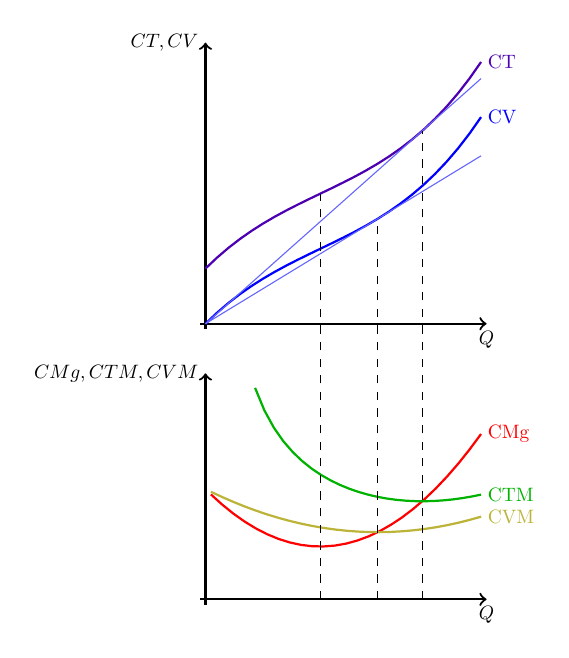
\begin{tikzpicture}[
			scale = 0.7,
			every node/.style = {scale =0.7},
			declare function = {
				cv(\x) = \x - (1/4)*\x^2 + (1/25)*\x^3;
				cf(\x) = 1;
				ct(\x) = cv(\x) + cf(\x);
				cmg(\x) = 1 - (2/4)*\x + (3/25)*\x^2;
				ctm(\x) = ct(\x)/\x;
				cvm(\x) = cv(\x)/\x;
			}
		]

		\draw[->,thick] (-0.1,0) -- (5.1,0) node[below]{$Q$};
		\draw[->,thick] (0,-0.1) -- (0,5.1) node[left]{$CT,CV$};

		\onslide<2->{
			\draw[blue,thick,domain=0:5,variable=\x] plot (\x,{cv(\x)});
			\draw[blue!60!white,domain=0:5,variable=\x] plot (\x,{\x*cvm(25/8)});	
			\draw[blue](5,{cv(5)})node[right]{CV};
		}

		\onslide<3->{
			\draw[blue!70!red,thick,domain=0:5,variable=\x] plot (\x,{ct(\x)});
			\draw[blue!70!red](5,{ct(5)})node[right]{CT};
			\draw[blue!60!white,domain=0:5,variable=\x] plot (\x,{\x*ctm(3.9330669)});
		}

		%===============================================================

		\draw[->,thick] (-0.1,-5) -- (5.1,-5) node[below]{$Q$};
		\draw[->,thick] (0,-5.1) -- (0,-0.9) node[left]{$CMg,CTM,CVM$};

		\draw[red,thick,domain=0.1:5,variable=\x] plot (\x,{2*cmg(\x)-5});
		\draw[green!70!black,thick,domain=0.9:5,variable=\x] plot (\x,{2*ctm(\x)-5});
		\draw[yellow!70!black,thick,domain=0.1:5,variable=\x] plot (\x,{2*cvm(\x)-5});

		\draw[red](5,{2*cmg(5)-5})node[right]{CMg};
		\draw[green!70!black](5,{2*ctm(5)-5})node[right]{CTM};
		\draw[yellow!70!black](5,{2*cvm(5)-5})node[right]{CVM};
		
		%===============================================================		

		\onslide<4->{
			\draw[dashed] ({25/12},-5) -- ({25/12},{ct(25/12)});
			\draw[dashed] ({25/8},-5) -- ({25/8},{cv(25/8)});
			\draw[dashed] ({3.9330669},-5) -- ({3.9330669},{ct(3.9330669)});
		}
		\end{tikzpicture}
	\end{center}
\end{frame}

\begin{frame}
	\frametitle{Sistematizando ideias}
	\begin{itemize}
		\item Para o output em que o $MPL$ \'e m\'aximo, o $CMg$ \'e m\'inimo \pause
		\item O $MPL$ \'e m\'aximo no ponto de inflex\~ao da fun\c c\~ao de produto total \pause
		\item O $CMg$ \'e m\'inimo no ponto de inflex\~ao da curva de custo total (custo vari\'avel)
		\item Para o output em que o $APL$ \'e m\'aximo, o $CVM$ \'e m\'inimo
	\end{itemize}
\end{frame}

\begin{frame}
	\frametitle{Rela\c c\~ao entre MPL e CMg}

	\begin{align*}
		CMg = \frac{\Delta CT}{\Delta Q} = \frac{\Delta CT}{\Delta L}\frac{\Delta L}{\Delta Q}=\frac{\Delta CT}{\Delta L}\times\frac{1}{\left(\frac{\Delta Q}{\Delta L}\right)}=\frac{\left(\frac{\Delta CT}{\Delta L}\right)}{MPL}
	\end{align*}

	\begin{align*}
		CVM = \frac{CV}{Q} = \frac{CV}{L}\frac{L}{Q}=\frac{CV}{L}\frac{1}{\left(\frac{Q}{L}\right)}=\frac{\left(\frac{CV}{L}\right)}{APL}
	\end{align*}
	\onslide<2->{
		Para o caso do exemplo que temos ussado nesta aula, $CV=wL$ e tamb\'em $\frac{\Delta CT}{\Delta L}=\frac{\Delta CV}{\Delta L}=w$ pelo que temos
		\begin{align*}
			CMg = \frac{w}{MPL}\\
			CVM = \frac{w}{APL}
		\end{align*}

	}
\end{frame}


\begin{frame}
	\frametitle{Escolha \'optima de uma empresa}
	\begin{itemize}
		\item O objectivo ser\'a sempre produzir de forma a ter lucro m\'aximo \pause
		\item A forma de atingir esse objectivo depende do contexto de mercado em que a empresa est\'a instalada \pause
		\item A estrutura de mercado afecta o controlo que a empresa tem sobre o pre\c co a que vende
	\end{itemize}
\end{frame}

\begin{frame}
	\frametitle{Estruturas de Mercado}
	\begin{center}
		{\scriptsize
		\renewcommand{\arraystretch}{3}
		\begin{tabular}{|c|c|c|c|c|c|}
			\hline
			\multicolumn{2}{|c|}{\cellcolor{blue!10!white} \multirow{2}{*}{\parbox{2cm}{\centering Estruturas de Mercado}}} & \multicolumn{4}{c|}{\cellcolor{blue!10!white} N\textsuperscript{o} de Agentes Econ\'omicos do lado da Oferta} \\ \cline{3-6}
			\multicolumn{2}{|c|}{\cellcolor{blue!10!white}} 																  &\cellcolor{blue!30!white} Muitos &\cellcolor{blue!30!white} Poucos &\cellcolor{blue!30!white} Dois &\cellcolor{blue!30!white} Um \\\hline
			\cellcolor{blue!10!white}&\cellcolor{blue!30!white} Muitos & \parbox{2.2cm}{\centering Mercados Concorrenciais} & Oligop\'olio & Duop\'olio & Monop\'olio \\ \cline{2-6}
			\cellcolor{blue!10!white}&\cellcolor{blue!30!white} Poucos & Oligops\'onio & \multicolumn{3}{c|}{\multirow{3}{*}{\parbox{4cm}{\centering Negocia\c c\~ao Estrat\'egica entre Agentes Econ\'omicos}}} \\ \cline{2-3}
			\cellcolor{blue!10!white}&\cellcolor{blue!30!white} Dois   & Duops\'onio   & \multicolumn{3}{c|}{} \\ \cline{2-3}
			\cellcolor{blue!10!white}\multirow{-4}{*}{\parbox{2cm}{\centering N\textsuperscript{o} de Agentes Econ\'omicos do lado da Procura}}&\cellcolor{blue!30!white} Um     & Monops\'onio  & \multicolumn{3}{c|}{} \\ \hline
		\end{tabular}
		}
	\end{center}
\end{frame}

\begin{frame}
	\frametitle{Estruturas de Mercado}
	\begin{center}
		{\scriptsize
		\renewcommand{\arraystretch}{3}
		\begin{tabular}{|c|c|c|c|c|c|}
			\hline
			\multicolumn{2}{|c|}{\cellcolor{blue!10!white} \multirow{2}{*}{\parbox{2cm}{\centering Estruturas de Mercado}}} & \multicolumn{4}{c|}{\cellcolor{blue!10!white} N\textsuperscript{o} de Agentes Econ\'omicos do lado da Oferta} \\ \cline{3-6}
			\multicolumn{2}{|c|}{\cellcolor{blue!10!white}} 																  &\cellcolor{blue!30!white} Muitos &\cellcolor{blue!30!white} Poucos &\cellcolor{blue!30!white} Dois &\cellcolor{blue!30!white} Um \\\hline
			\cellcolor{blue!10!white}&\cellcolor{blue!30!white} Muitos & \parbox{2.2cm}{\centering Mercados Concorrenciais} & Oligop\'olio & Duop\'olio & \cellcolor{red}{\color{white}\textbf{Monop\'olio}} \\ \cline{2-6}
			\cellcolor{blue!10!white}&\cellcolor{blue!30!white} Poucos & Oligops\'onio & \multicolumn{3}{c|}{\multirow{3}{*}{\parbox{4cm}{\centering Negocia\c c\~ao Estrat\'egica entre Agentes Econ\'omicos}}} \\ \cline{2-3}
			\cellcolor{blue!10!white}&\cellcolor{blue!30!white} Dois   & Duops\'onio   & \multicolumn{3}{c|}{} \\ \cline{2-3}
			\cellcolor{blue!10!white}\multirow{-4}{*}{\parbox{2cm}{\centering N\textsuperscript{o} de Agentes Econ\'omicos do lado da Procura}}&\cellcolor{blue!30!white} Um     & \cellcolor{red}{\color{white}\textbf{Monops\'onio}}  & \multicolumn{3}{c|}{} \\ \hline
		\end{tabular}
		}
	\end{center}
\end{frame}

\begin{frame}
	\frametitle{Estruturas de Mercado}
	\begin{center}
		{\scriptsize
		\renewcommand{\arraystretch}{3}
		\begin{tabular}{|c|c|c|c|c|c|}
			\hline
			\multicolumn{2}{|c|}{\cellcolor{blue!10!white} \multirow{2}{*}{\parbox{2cm}{\centering Estruturas de Mercado}}} & \multicolumn{4}{c|}{\cellcolor{blue!10!white} N\textsuperscript{o} de Agentes Econ\'omicos do lado da Oferta} \\ \cline{3-6}
			\multicolumn{2}{|c|}{\cellcolor{blue!10!white}} 																  &\cellcolor{blue!30!white} Muitos &\cellcolor{blue!30!white} Poucos &\cellcolor{blue!30!white} Dois &\cellcolor{blue!30!white} Um \\\hline
			\cellcolor{blue!10!white}&\cellcolor{blue!30!white} Muitos & \cellcolor{green!70!black}\parbox{2.2cm}{\color{white}\centering \textbf{Mercados Concorrenciais}} & Oligop\'olio & Duop\'olio & \cellcolor{green!70!black}{\color{white}\textbf{Monop\'olio}} \\ \cline{2-6}
			\cellcolor{blue!10!white}&\cellcolor{blue!30!white} Poucos & Oligops\'onio & \multicolumn{3}{c|}{\multirow{3}{*}{\parbox{4cm}{\centering Negocia\c c\~ao Estrat\'egica entre Agentes Econ\'omicos}}} \\ \cline{2-3}
			\cellcolor{blue!10!white}&\cellcolor{blue!30!white} Dois   & Duops\'onio   & \multicolumn{3}{c|}{} \\ \cline{2-3}
			\cellcolor{blue!10!white}\multirow{-4}{*}{\parbox{2cm}{\centering N\textsuperscript{o} de Agentes Econ\'omicos do lado da Procura}}&\cellcolor{blue!30!white} Um     & Monops\'onio  & \multicolumn{3}{c|}{} \\ \hline
		\end{tabular}
		}
	\end{center}
\end{frame}


\begin{frame}
	\frametitle{Concorr\^encia}
	\begin{itemize}
		\item Em concorr\^encia perfeita, a empresa individualmente n\~ao tem controlo nenhum sobre o pre\c co unit\'ario de venda do produto
		\item Em monop\'olio, a empresa tem controlo m\'aximo sobre o pre\c co
		\item O grau de controlo sobre o pre\c co depende do poder de mercado da empresa
	\end{itemize}
\end{frame}

\begin{frame}
	\frametitle{Concorr\^encia Perfeita (curto prazo)}
	Hip\'oteses:
	\begin{itemize}
		\item Mercado atomizado: cada agente econ\'omico representa um infinit\'esimo do mercado, seja do lado da procura, seja do lado da oferta
		\item O produto transacionado \'e homog\'eneo
		\item Individualmente, cada empresa n\~ao tem poder de mercado e toma o pre\c co unit\'ario do produto como uma vari\'avel ex\'ogena (price takers)
		\item Livre entrada e sa\'ida do mercado
		\item Informa\c c\~ao Perfeita
	\end{itemize}
\end{frame}
\section{Oferta}
\begin{frame}
	\frametitle{Custo M\'edio e Lucro}
	Em geral:
	\begin{align*}
		\text{Lucro} &= \text{Receita Total} - \text{Custo Total}\\
		\Pi &= RT - CT \\
		\Pi &= PQ-CF-CV \\
		\Pi &= Q(P-CTM) = Q(P-CVM-CFM)
	\end{align*}

	Se o pre\c co unit\'ario de venda do bem for suficientemente grande, $P>CTM$, a empresa ter\'a lucro, caso contr\'ario, ter\'a prejuizo.
\end{frame}

\begin{frame}
	\frametitle{Custo M\'edio e Lucro}
	\[\Pi=Q(P-CVM-CFM)\]
	Quando h\'a preju\'izo, ele pode ter naturezas muito diferentes:
	\begin{itemize}
		\item $P-CVM>0$, mas inferior a $CFM$: a receita \'e suficiente para pagar os factores vari\'aveis, mas n\~ao chega para a totalidade dos factores fixos, havendo preju\'izo a curto prazo
		\item $P-CVM<0$, a empresa \'e insustent\'avel: as receitas nem sequer cobrem o custo vari\'avel
	\end{itemize}
\end{frame}

\begin{frame}
	\frametitle{Maximiza\c c\~ao do Lucro Econ\'omico; Escolha \'Optima da empresa}
	Cada empresa pretende encontrar a quantidade a produzir tal que: \[Max \Pi = RT-CT\]
	Sendo:\[\Pi=pQ_i-CV(Q_i)-CF\]
	CPO:\ \(\frac{d\Pi}{dQ_i} = 0 \Leftrightarrow p-CV'=0\Leftrightarrow p=CMg\) \\
	CSO:\ \(\frac{d^2\Pi}{dQ_i^2} < 0 \Leftrightarrow -\frac{dCMg}{dQ_i}<0\Leftrightarrow\frac{dCMg}{dQ_i}>0 \Leftrightarrow \text{CMg crescente}\)
\end{frame}

\begin{frame}
	\frametitle{Maximiza\c c\~ao do Lucro}
	A quantidade \'optima a produzir \'e tal que $p=CMg$ na zona ascendente da curva de $CMg$. Dado um pre\c co $P^*$, ent\~ao a quantidade \'optima \'e $Q_i^*$.
	\begin{center}
		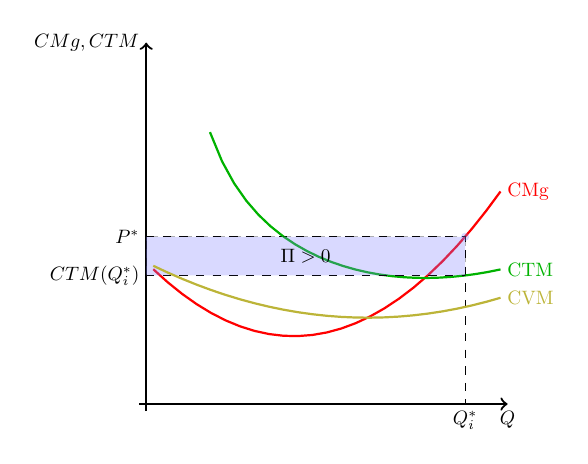
\begin{tikzpicture}[
			scale = 0.9,
			every node/.style = {scale =0.7},
			declare function = {
				cv(\x) = \x - (1/4)*\x^2 + (1/25)*\x^3;
				cf(\x) = 1;
				ct(\x) = cv(\x) + cf(\x);
				cmg(\x) = 1 - (2/4)*\x + (3/25)*\x^2;
				ctm(\x) = ct(\x)/\x;
				cvm(\x) = cv(\x)/\x;
			}
		]

			\def\p{4.5}

			\draw[->,thick] (-0.1,-0) -- (5.1,-0) node[below]{$Q$};
			\draw[->,thick] (0,-0.1) -- (0,5.1) node[left]{$CMg,CTM$};

			\onslide<2->{
				\draw[red,thick,domain=0.1:5,variable=\x] plot (\x,{2*cmg(\x)-0});
				\draw[red](5,{2*cmg(5)-0})node[right]{CMg};
			}
			\onslide<3->{
				\draw[dashed] (0,{2*cmg(\p)})node[left]{$P^*$} -- (\p,{2*cmg(\p)}) -- (\p,0)node[below]{$Q_i^*$};		
			}

			\onslide<4->{
				\draw[green!70!black,thick,domain=0.9:5,variable=\x] plot (\x,{2*ctm(\x)-0});
				\draw[green!70!black](5,{2*ctm(5)-0})node[right]{CTM};
			}

			\onslide<5->{
				\draw[dashed] (0,{2*ctm(\p)})node[left]{$CTM(Q_i^*)$} -- (\p,{2*ctm(\p)});		
			}

			\onslide<6->{
				\draw[dashed,fill=blue!50!white,opacity=0.3] (0,{2*ctm(\p)}) -- (\p,{2*ctm(\p)}) --(\p,{2*cmg(\p)}) node[circle,fill,inner sep = 1.5]{} -- (0,{2*cmg(\p)}) -- (0,{2*ctm(\p)});
				\draw({\p/2},{(2*cmg(\p)+2*ctm(\p))/2}) node{$\Pi>0$};
			}
			
			\onslide<7->{
				\draw[yellow!70!black,thick,domain=0.1:5,variable=\x] plot (\x,{2*cvm(\x)-0});
				\draw[yellow!70!black](5,{2*cvm(5)-0})node[right]{CVM};
			}			

		\end{tikzpicture}
	\end{center}
\end{frame}


\begin{frame}
	\frametitle{Maximiza\c c\~ao do Lucro}
	A quantidade \'optima a produzir \'e tal que $p=CMg$ na zona ascendente da curva de $CMg$. Dado um pre\c co $P^*$, ent\~ao a quantidade \'optima \'e $Q_i^*$ e h\'a um preju\'izo!
	\begin{center}
		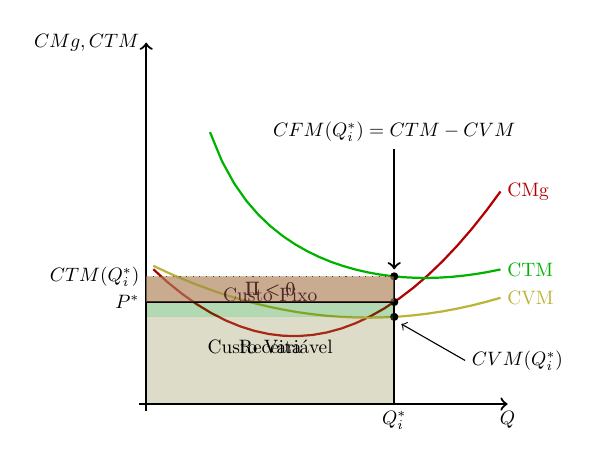
\begin{tikzpicture}[
			scale = 0.9,
			every node/.style = {scale =0.7},
			declare function = {
				cv(\x) = \x - (1/4)*\x^2 + (1/25)*\x^3;
				cf(\x) = 1;
				ct(\x) = cv(\x) + cf(\x);
				cmg(\x) = 1 - (2/4)*\x + (3/25)*\x^2;
				ctm(\x) = ct(\x)/\x;
				cvm(\x) = cv(\x)/\x;
			}
		]

			\def\p{3.5}

			\draw[->,thick] (-0.1,-0) -- (5.1,-0) node[below]{$Q$};
			\draw[->,thick] (0,-0.1) -- (0,5.1) node[left]{$CMg,CTM$};

			
			\draw[red!70!black,thick,domain=0.1:5,variable=\x] plot (\x,{2*cmg(\x)-0});
			\draw[red!70!black](5,{2*cmg(5)-0})node[right]{CMg};	
			

			\onslide<2->{
				\draw[dotted] (0,{2*cmg(\p)})node[left]{$P^*$} -- (\p,{2*cmg(\p)});
			}

			\onslide<3->{
				\draw[dotted] (\p,0)node[below]{$Q_i^*$}--(\p,{2*cmg(\p)})node[circle,fill,inner sep=1.5pt]{};
			}

			\onslide<4->{
				 \draw[green!70!black,thick,domain=0.9:5,variable=\x] plot (\x,{2*ctm(\x)-0});	
				 \draw[green!70!black](5,{2*ctm(5)-0})node[right]{CTM};
				 
				 \draw[dotted] (\p,{2*cmg(\p)}) -- (\p,{2*ctm(\p)})node[circle,fill,inner sep=1.5pt]{};
				 \draw[dotted] (0,{2*ctm(\p)})node[left]{$CTM(Q_i^*)$} -- (\p,{2*ctm(\p)});
			}

			\onslide<5-9>{
				\draw({\p/2},{(2*cmg(\p)+2*ctm(\p))/2}) node{$\Pi<0$};
				\draw[draw=none,fill=red!50!white,opacity=0.3] (0,{2*ctm(\p)}) -- (\p,{2*ctm(\p)}) --(\p,{2*cmg(\p)}) -- (0,{2*cmg(\p)}) -- (0,{2*ctm(\p)});
			}

			\onslide<6->{
				\draw[yellow!70!black,thick,domain=0.1:5,variable=\x] plot (\x,{2*cvm(\x)-0});
				\draw[yellow!70!black](5,{2*cvm(5)-0})node[right]{CVM};
			}

			\onslide<7->{
				\draw[<-] (\p+0.1,{2*cvm(\p)-0.1}) -- ({\p+1},{cvm(\p)}) node[right]{$CVM(Q_i^*)$};
				\draw[] (\p,{2*cvm(\p)}) node[circle,fill,inner sep=1.5pt]{};
			}

			\onslide<8->{
				\draw[<-,thick] ({\p},{2*ctm(\p)+0.1}) -- ({\p},{4*ctm(\p)})node[above]{$CFM(Q_i^*)=CTM-CVM$};
				\draw[thick] (\p,{2*cvm(\p)}) -- (\p,{2*ctm(\p)});
			}

			\onslide<9->{
				\draw[thick,red] (\p,{2*cvm(\p)}) -- (\p,{2*cmg(\p)});	
			}

			\onslide<10-11>{
				\draw[draw=none,fill=green!50!black,opacity=0.3] (0,{2*ctm(\p)}) -- (\p,{2*ctm(\p)}) --(\p,{2*cvm(\p)}) -- (0,{2*cvm(\p)}) -- (0,{2*ctm(\p)});

				\draw[draw=none,fill=yellow!50!black,opacity=0.3] (0,{2*cvm(\p)}) -- (\p,{2*cvm(\p)}) --(\p,0) -- (0,0) -- (0,{2*cvm(\p)});
			}

			\onslide<10>{
				\draw({\p/2},{(2*cmg(\p)+2*ctm(\p))/2.1}) node{Custo Fixo};
				\draw({\p/2},{(2*cmg(\p)+2*ctm(\p))/4}) node{Custo Vari\'avel};
			}

			\onslide<11>{
				\draw[thick] (0,0) -- (\p,0) -- (\p,{2*cmg(\p)}) -- (0,{2*cmg(\p)}) -- (0,0);
				\draw({\p/2},{(2*cmg(\p)+2*ctm(\p))/4}) node{Receita};
			}

			\onslide<12>{
				\draw({\p/2},{(2*cmg(\p)+2*ctm(\p))/2}) node{$\Pi<0$};
				\draw[draw=none,fill=red!50!white,opacity=0.3] (0,{2*ctm(\p)}) -- (\p,{2*ctm(\p)}) --(\p,{2*cmg(\p)}) -- (0,{2*cmg(\p)}) -- (0,{2*ctm(\p)});
			}

		\end{tikzpicture}
	\end{center}
\end{frame}


\begin{frame}
	\frametitle{Maximiza\c c\~ao do Lucro}
	A quantidade \'optima a produzir \'e tal que $p=CMg$ na zona ascendente da curva de $CMg$. Dado um pre\c co $P^*$, ent\~ao a quantidade \'optima \'e $Q_i^*$ e h\'a um preju\'izo superior a $CF$!
	\begin{center}
		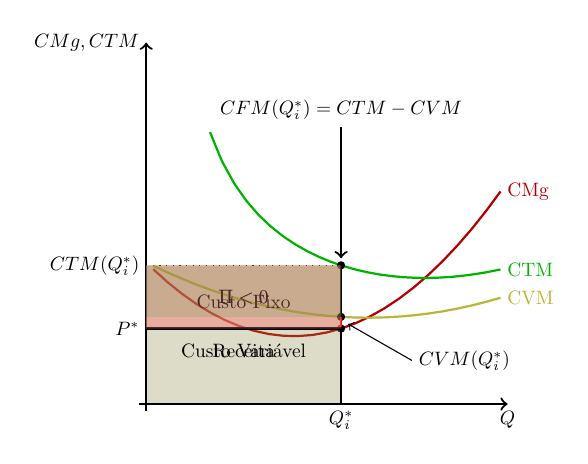
\begin{tikzpicture}[
			scale = 0.9,
			every node/.style = {scale =0.7},
			declare function = {
				cv(\x) = \x - (1/4)*\x^2 + (1/25)*\x^3;
				cf(\x) = 1;
				ct(\x) = cv(\x) + cf(\x);
				cmg(\x) = 1 - (2/4)*\x + (3/25)*\x^2;
				ctm(\x) = ct(\x)/\x;
				cvm(\x) = cv(\x)/\x;
			}
		]

			\def\p{2.75}

			\draw[->,thick] (-0.1,-0) -- (5.1,-0) node[below]{$Q$};
			\draw[->,thick] (0,-0.1) -- (0,5.1) node[left]{$CMg,CTM$};

			
			\draw[red!70!black,thick,domain=0.1:5,variable=\x] plot (\x,{2*cmg(\x)-0});
			\draw[red!70!black](5,{2*cmg(5)-0})node[right]{CMg};	
			

			\onslide<2->{
				\draw[dotted] (0,{2*cmg(\p)})node[left]{$P^*$} -- (\p,{2*cmg(\p)});
			}

			\onslide<3->{
				\draw[dotted] (\p,0)node[below]{$Q_i^*$}--(\p,{2*cmg(\p)})node[circle,fill,inner sep=1.5pt]{};
			}

			\onslide<4->{
				 \draw[green!70!black,thick,domain=0.9:5,variable=\x] plot (\x,{2*ctm(\x)-0});	
				 \draw[green!70!black](5,{2*ctm(5)-0})node[right]{CTM};
				 
				 \draw[dotted] (\p,{2*cmg(\p)}) -- (\p,{2*ctm(\p)})node[circle,fill,inner sep=1.5pt]{};
				 \draw[dotted] (0,{2*ctm(\p)})node[left]{$CTM(Q_i^*)$} -- (\p,{2*ctm(\p)});
			}

			\onslide<5-9>{
				\draw({\p/2},{(2*cmg(\p)+2*ctm(\p))/2}) node{$\Pi<0$};
				\draw[draw=none,fill=red!50!white,opacity=0.3] (0,{2*ctm(\p)}) -- (\p,{2*ctm(\p)}) --(\p,{2*cmg(\p)}) -- (0,{2*cmg(\p)}) -- (0,{2*ctm(\p)});
			}

			\onslide<6->{
				\draw[yellow!70!black,thick,domain=0.1:5,variable=\x] plot (\x,{2*cvm(\x)-0});
				\draw[yellow!70!black](5,{2*cvm(5)-0})node[right]{CVM};
			}

			\onslide<7->{
				\draw[<-] (\p+0.1,{2*cvm(\p)-0.1}) -- ({\p+1},{cvm(\p)}) node[right]{$CVM(Q_i^*)$};
				\draw[] (\p,{2*cvm(\p)}) node[circle,fill,inner sep=1.5pt]{};
			}

			\onslide<8->{
				\draw[<-,thick] ({\p},{2*ctm(\p)+0.1}) -- ({\p},{4*ctm(\p)})node[above]{$CFM(Q_i^*)=CTM-CVM$};
				\draw[thick] (\p,{2*cvm(\p)}) -- (\p,{2*ctm(\p)});
			}

			\onslide<9->{
				\draw[thick,red] (\p,{2*cvm(\p)}) -- (\p,{2*cmg(\p)});	
			}

			\onslide<10-11>{
				\draw[draw=none,fill=green!50!black,opacity=0.3] (0,{2*ctm(\p)}) -- (\p,{2*ctm(\p)}) --(\p,{2*cvm(\p)}) -- (0,{2*cvm(\p)}) -- (0,{2*ctm(\p)});

				\draw[draw=none,fill=yellow!50!black,opacity=0.3] (0,{2*cvm(\p)}) -- (\p,{2*cvm(\p)}) --(\p,0) -- (0,0) -- (0,{2*cvm(\p)});
			}

			\onslide<10>{
				\draw({\p/2},{(2*cmg(\p)+2*ctm(\p))/2.1}) node{Custo Fixo};
				\draw({\p/2},{(2*cmg(\p)+2*ctm(\p))/4}) node{Custo Vari\'avel};
			}

			\onslide<11>{
				\draw[thick] (0,0) -- (\p,0) -- (\p,{2*cmg(\p)}) -- (0,{2*cmg(\p)}) -- (0,0);
				\draw({\p/2},{(2*cmg(\p)+2*ctm(\p))/4}) node{Receita};
			}

			\onslide<12>{
				\draw({\p/2},{(2*cmg(\p)+2*ctm(\p))/2}) node{$\Pi<0$};
				\draw[draw=none,fill=red!50!white,opacity=0.3] (0,{2*ctm(\p)}) -- (\p,{2*ctm(\p)}) --(\p,{2*cmg(\p)}) -- (0,{2*cmg(\p)}) -- (0,{2*ctm(\p)});
			}

		\end{tikzpicture}
	\end{center}
\end{frame}

\begin{frame}
	\frametitle{Lucro ou Preju\'izo?}
	\begin{itemize}
		\setlength{\itemsep}{15pt}
		\item $\Pi^* = P^*Q^*-CTM(Q_i^*)Q_i^* = RT^*-CT^*$
		\item $\Pi^*>0\Leftrightarrow P^*Q_i^*>CTM(Q_i^*)Q_i^*\Leftrightarrow P^*>CTM$
		\item $\Pi^*<0\Leftrightarrow P^* < CTM \Rightarrow$ o preju\'izo \'e inferior a $CF$
		\item $P^*<CMV\Rightarrow\Pi^*<-CF\Rightarrow$ Encerrar!, e ter\'a apenas $CF$ como preju\'izo
	\end{itemize}
\end{frame}


\begin{frame}
	\frametitle{Rendibilidade e Encerramento a curto prazo}

	\begin{center}
		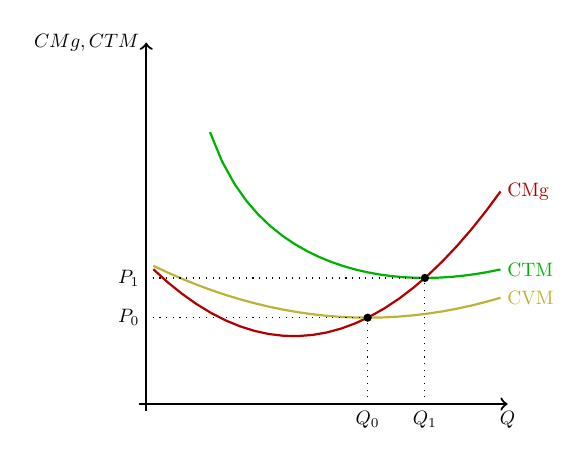
\begin{tikzpicture}[
			scale = 0.9,
			every node/.style = {scale =0.7},
			declare function = {
				cv(\x) = \x - (1/4)*\x^2 + (1/25)*\x^3;
				cf(\x) = 1;
				ct(\x) = cv(\x) + cf(\x);
				cmg(\x) = 1 - (2/4)*\x + (3/25)*\x^2;
				ctm(\x) = ct(\x)/\x;
				cvm(\x) = cv(\x)/\x;
			}
		]

			\def\p{3.9330669}
			\def\q{25/8}

			\draw[->,thick] (-0.1,-0) -- (5.1,-0) node[below]{$Q$};
			\draw[->,thick] (0,-0.1) -- (0,5.1) node[left]{$CMg,CTM$};

			
			\draw[red!70!black,thick,domain=0.1:5,variable=\x] plot (\x,{2*cmg(\x)-0});
			\draw[red!70!black](5,{2*cmg(5)-0})node[right]{CMg};	
			
			\draw[green!70!black,thick,domain=0.9:5,variable=\x] plot (\x,{2*ctm(\x)-0});	
		 	\draw[green!70!black](5,{2*ctm(5)-0})node[right]{CTM};
			 
			\draw[yellow!70!black,thick,domain=0.1:5,variable=\x] plot (\x,{2*cvm(\x)-0});
			\draw[yellow!70!black](5,{2*cvm(5)-0})node[right]{CVM};

			\onslide<3->{
				\draw[dotted] (0,{2*cmg(\q)})node[left]{$P_0$} -- (\q,{2*cmg(\q)});
				\draw[dotted] (\q,0)node[below]{$Q_0$}--(\q,{2*cmg(\q)})node[circle,fill,inner sep=1.5pt]{};
			}

			\onslide<3->{
				\draw[dotted] (0,{2*cmg(\p)})node[left]{$P_1$} -- (\p,{2*cmg(\p)});
				\draw[dotted] (\p,0)node[below]{$Q_1$}--(\p,{2*cmg(\p)})node[circle,fill,inner sep=1.5pt]{};
			}

		\end{tikzpicture}
	\end{center}
\end{frame}

\begin{frame}
	\frametitle{Rendibilidade e Encerramento}
	\begin{itemize}
		\setlength{\itemsep}{15pt}
		\item Para pre\c cos abaixo de $P_1$ a empresa ter\'a preju\'izo, produzindo a quantidade tal que $P=CMg$, j\'a que $P<CTM$. {\color{red} $P_1$ identifica o limiar de rendibilidade da empresa}
		\item Para pre\c cos entre $P_0$ e $P_1$ a empresa ter\'a um preju\'izo inferior a $CF$, produzindo a quantidade tal que $P=CMg$, j\'a que $P<CVM$, pelo que se deve manter em funcionamento.
	\end{itemize}
\end{frame}

\begin{frame}
	\frametitle{Rendibilidade e Encerramento}
	\begin{itemize}
		\setlength{\itemsep}{15pt}
		\item Para pre\c cos abaixo de $P_0$ a empresa ter\'a preju\'izo superior a $CF$, produzindo a quantidade tal que $P=CMg$, j\'a que $P<CVM$. {\color{red} $P_0$ identifica o limiar de encerramento da empresa e $Q_0$ corresponde ao \'optimo t\'ecnico.}
		\item {\color{red} Nesta situa\c c\~ao, encerrando, a empresa enfrenta apenas o custo de oportunidade dos factores fixos: o custo fixo!}
	\end{itemize}
\end{frame}

\begin{frame}
	\frametitle{Oferta individual da Empresa: $S_i$ (curto prazo)}

	\begin{center}
		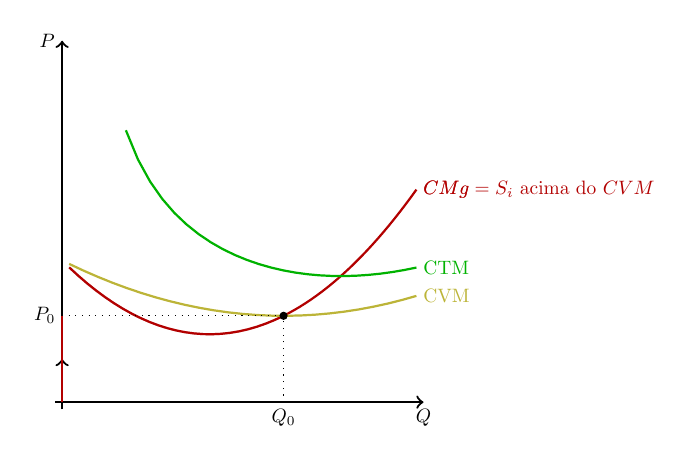
\begin{tikzpicture}[
			scale = 0.9,
			every node/.style = {scale =0.7},
			declare function = {
				cv(\x) = \x - (1/4)*\x^2 + (1/25)*\x^3;
				cf(\x) = 1;
				ct(\x) = cv(\x) + cf(\x);
				cmg(\x) = 1 - (2/4)*\x + (3/25)*\x^2;
				ctm(\x) = ct(\x)/\x;
				cvm(\x) = cv(\x)/\x;
			}
		]

			\def\p{3.9330669}
			\def\q{25/8}

			\draw[->,thick] (-0.1,-0) -- (5.1,-0) node[below]{$Q$};
			\draw[->,thick] (0,{cvm(\q)}) -- (0,5.1) node[left]{$P$};
			
			\onslide<1>{
				\draw[->,thick] (0,-0.1) -- (0,{cvm(\q)});
			}

			\draw[red!70!black,thick,domain=\q:5,variable=\x] plot (\x,{2*cmg(\x)-0});

			\onslide<1>{
				\draw[red!70!black,thick,domain=0.1:\q,variable=\x] plot (\x,{2*cmg(\x)-0});
			}

			\onslide<2->{
				\draw[red!70!black,opacity=0.3,thick,domain=0.1:\q,variable=\x] plot (\x,{2*cmg(\x)-0});
			}

			\onslide<1>{
				\draw[red!70!black](5,{2*cmg(5)-0})node[right]{$CMg$};	
			}

			\onslide<2->{
				\draw[red!70!black](5,{2*cmg(5)-0})node[right]{$CMg=S_i$ acima do $CVM$};
			}

			\draw[green!70!black,thick,domain=0.9:5,variable=\x] plot (\x,{2*ctm(\x)-0});	
		 	\draw[green!70!black](5,{2*ctm(5)-0})node[right]{CTM};
			 
			\draw[yellow!70!black,thick,domain=0.1:5,variable=\x] plot (\x,{2*cvm(\x)-0});
			\draw[yellow!70!black](5,{2*cvm(5)-0})node[right]{CVM};

			\onslide<2->{
				\draw[dotted] (0,{2*cmg(\q)})node[left]{$P_0$} -- (\q,{2*cmg(\q)});
				\draw[dotted] (\q,0)node[below]{$Q_0$}--(\q,{2*cmg(\q)})node[circle,fill,inner sep=1.5pt]{};
				\draw[thick,red!70!black] (0,0) -- (0,{2*cvm(\q)});
			}

		\end{tikzpicture}
	\end{center}
\end{frame}

\begin{frame}
	\frametitle{Curva da oferta}
	\'E o conjunto de pares $(Q,P)$ que constituem a escolha \'optima de uma empresa, considerando fixos todos os factores ex\'ogenos \`a decis\~ao da empresa:

	\vspace{0.5cm}

	pre\c cos dos inputs, tecnologia,...
\end{frame}

\begin{frame}
	\frametitle{Lei da Oferta}
	Entre a quantidade oferecida de um bem e o pre\c co desse mesmo bem, existe uma rela\c c\~ao positiva: se o pre\c co aumenta, a quantidade oferecida aumenta, \emph{c\ae teris paribus}.
\end{frame}

\begin{frame}
	\frametitle{Lei da Oferta}
	A Lei da Oferta adv\'em de:

	\vspace{0.4cm}

		Custos marginais de produ\c c\~ao crescentes, consequ\^encia de rendimentos marginais decrescentes na produ\c c\~ao --- para produzir mais uma unidade o custo adicional \'e cada vez maior, logo o pre\c co que os produtores est\~ao dispostos a receber tem de aumentar com a quantidade.

\end{frame}

\begin{frame}
	\frametitle{Oferta}
	\begin{columns}
		\begin{column}{0.65\textwidth}
			\begin{center}
				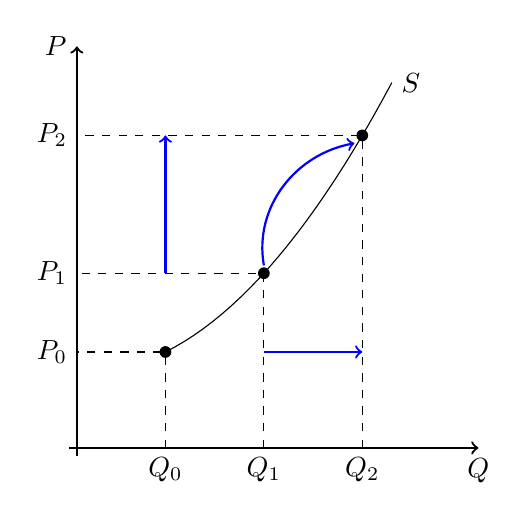
\begin{tikzpicture}[
					scale = 1,
					every node/.style = {scale =1},
					declare function = {
						s(\x) =  2*(1 - (2/4)*(\x+2) + (3/25)*(\x+2)^2); % > 25/8
					}
					]

				\def\q{25/8}
				\def\p{35/8}
				\def\r{45/8}

				\draw[->,thick] (-0.1,-0) -- (5.1,-0) node[below]{$Q$};
				\draw[->,thick] (0,-0.1) -- (0,5.1) node[left]{$P$};

				\draw[domain=(\q-2):4,variable=\x] plot (\x,{s(\x)});
				\draw(4,{s(4)}) node[right]{$S$};

				\draw[dashed]({\q-2},0)node[below]{$Q_0$} -- ({\q-2},{s(\q-2)})node[circle,fill,inner sep=1.5]{} -- (0,{s(\q-2)})node[left]{$P_0$};

				\onslide<2->{
					\draw[dashed]({\p-2},0)node[below]{$Q_1$} -- ({\p-2},{s(\p-2)})node[circle,fill,inner sep=1.5]{} -- (0,{s(\p-2)})node[left]{$P_1$};
				}

				\onslide<3->{
					\draw[dashed]({\r-2},0)node[below]{$Q_2$} -- ({\r-2},{s(\r-2)})node[circle,fill,inner sep=1.5]{} -- (0,{s(\r-2)})node[left]{$P_2$};
				}

				\onslide<4->{
					\draw[blue,thick,->] ({\q-2},{s(\p-2)}) -- ({\q-2},{s(\r-2)});
				}
				\onslide<5->{
					\draw[blue,thick,->] ({\p-2},{s(\q-2)}) -- ({\r-2},{s(\q-2)});
				}
				\onslide<6->{
					\draw[blue,thick,->] ({\p-2},{s(\p-2)+0.1}) to [out=100,in=190] ({\r-2-0.1},{s(\r-2)-0.1});
				}

				\end{tikzpicture}
			\end{center}
		\end{column}
		\begin{column}{0.3\textwidth}
			A Lei da Oferta descreve um movimento ao longo da curva:
			
			\vspace{0.5cm}

			A subida de pre\c co faz aumentar a quantidade oferecida, \emph{c\ae teris paribus}
		\end{column}
	\end{columns}
\end{frame}

\begin{frame}
	\frametitle{Inten\c c\~oes de Venda - Oferta}
	A quantidade de um bem que um produtor est\'a disposto a vender depende de:
	\begin{columns}
		\begin{column}{0.65\textwidth}
			\begin{itemize}
				\item \(p =\) pre\c co de venda {\color{red}(+)}
				\vspace{1cm}
				\item \(A =\) tecnologia de produ\c c\~ao{\color{red}(+)}
				\item \(r\ e\ w=\) pre\c co dos factores produtivos ($K$ e $L$){\color{red}(-)}
				\item $p_m$ = pre\c co de mat\'erias-primas{\color{red}(-)}
				\item $p_i$ = pre\c co de bens de consumo interm\'edio{\color{red}(-)}
				\item meteorologia (para o caso dos bens agr\'icolas){\color{red}(+)}
			\end{itemize}
		\end{column}
		\begin{column}{0.3\textwidth}
			\onslide<2->{
			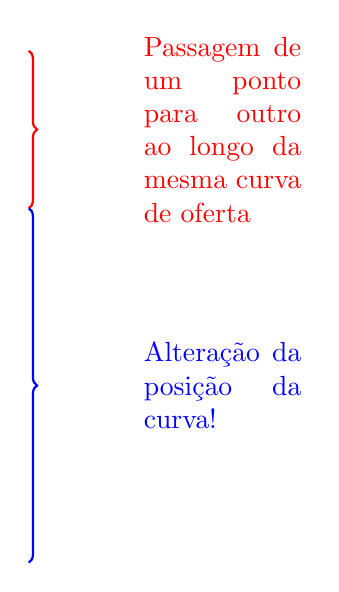
\begin{tikzpicture}[
				scale = 1,
				every node/.style = {scale = 1}
				]
				\draw [decorate,decoration={brace,mirror,amplitude=3pt},thick,red] (0,3) -- (0,5) node [midway,xshift=70pt] {\parbox{2cm}{Passagem de um ponto para outro ao longo da mesma curva de oferta}};
				
				\draw [decorate,decoration={brace,mirror,amplitude=3pt},thick,blue] (0,-1.5) -- (0,3) node [midway,xshift=70pt] {\parbox{2cm}{Altera\c c\~ao da posi\c c\~ao da curva!}};
			\end{tikzpicture}
			}
		\end{column}
	\end{columns}

\end{frame}

\begin{frame}
	\frametitle{Determinantes da Oferta}
	\begin{itemize}
		\item As vari\'aveis que levam \'a altera\c c\~ao da curva da oferta s\~ao ex\'ogenas \`a escolha da empresa e fazem com que as curvas de custo ou as curvas de produto se alterem.
		\item Havendo altera\c c\~ao das curvas de custo, h\'a altera\c c\~ao da curva da oferta.
		\item Uma altera\c c\~ao de pre\c co da venda, \emph{c\ae teris paribus} n\~ao faz alterar a curva da oferta, mas apenas se passa de um ponto na mesma curva.
	\end{itemize}
\end{frame}

\begin{frame}
	\frametitle{Oferta}
	\begin{itemize}
		\item \`A rela\c c\~ao funcional entre a quantidade oferecida de um bem e todas as vari\'aveis que a influenciam, chama-se \underline{Fun\c c\~ao Oferta:}\[Q_s=f(p,r,w,A,p_i,p_m,...)\]
		\item A curva de oferta obt\'em-se, estudando a rela\c c\~ao que existe entre a quantidade oferecida $Q_s$ e $p$, para valores dados das outras vari\'aveis (ex\'ogenas)
	\end{itemize}
	Diferentes valores das vari\'aveis ex\'ogenas geram curvas de oferta diferentes --- movimenta\c c\~ao da oferta no espa\c co ($Q,P$)
\end{frame}

\begin{frame}
	\frametitle{Expans\~ao da Oferta}
	\begin{center}
		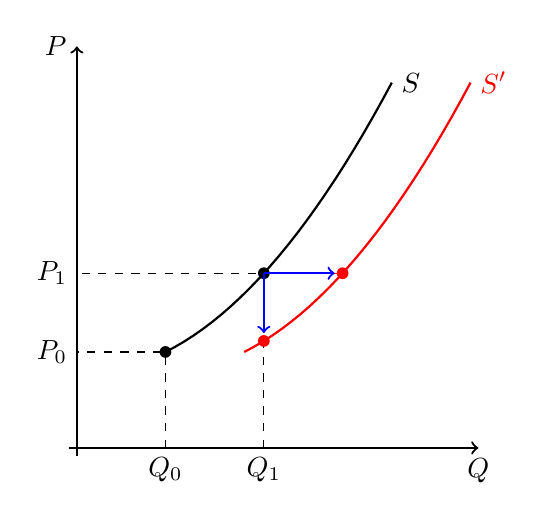
\begin{tikzpicture}[
			scale = 1,
			every node/.style = {scale =1},
			declare function = {
				s(\x) =  2*(1 - (2/4)*(\x+2) + (3/25)*(\x+2)^2); % > 25/8
			}
			]

		\def\q{25/8}
		\def\p{35/8}
		\def\r{45/8}

		\draw[->,thick] (-0.1,-0) -- (5.1,-0) node[below]{$Q$};
		\draw[->,thick] (0,-0.1) -- (0,5.1) node[left]{$P$};

		\draw[thick,domain=(\q-2):4,variable=\x] plot (\x,{s(\x)});
		\draw({5-1},{s(5-1)}) node[right]{$S$};

		\draw[dashed]({\q-2},0)node[below]{$Q_0$} -- ({\q-2},{s(\q-2)})node[circle,fill,inner sep=1.5]{} -- (0,{s(\q-2)})node[left]{$P_0$};

		\onslide<2->{
			\draw[thick,red,domain=(\q-1):5,variable=\x] plot (\x,{s(\x-1)});
			\draw[red](5,{s(5-1)}) node[right]{$S'$};
			\draw[dashed]({\p-2},0)node[below]{$Q_1$} -- ({\p-2},{s(\p-2)})node[circle,fill,inner sep=1.5]{} -- (0,{s(\p-2)})node[left]{$P_1$};
		}

		\onslide<3->{
			\draw[dashed,red]({\p-2},{s(\p-2)}) -- ({\p-1},{s(\p-2)})node[circle,fill,inner sep=1.5]{};

			\draw[red] ({\p-2},{s(\p-3)}) node[circle,fill,inner sep=1.5]{};

			\draw[blue,thick,->] ({\p-2},{s(\p-2)}) -- ({\p-1-0.1},{s(\p-2)});
			\draw[blue,thick,->] ({\p-2},{s(\p-2)}) -- ({\p-2},{s(\p-3)+0.1});
		}

		\end{tikzpicture}
	\end{center}
	\onslide<4->{Que altera\c c\~ao de vari\'aveis ex\'ogenas poderia estar na origem da desloca\c c\~ao da oferta?}
\end{frame}

\begin{frame}
	\frametitle{Expans\~ao da Oferta}
	\begin{center}
		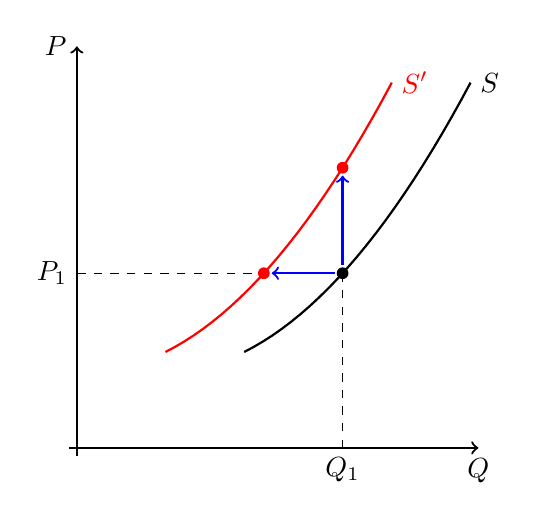
\begin{tikzpicture}[
			scale = 1,
			every node/.style = {scale =1},
			declare function = {
				s(\x) =  2*(1 - (2/4)*(\x+2) + (3/25)*(\x+2)^2); % > 25/8
			}
			]

		\def\q{25/8}
		\def\p{35/8}
		\def\r{45/8}

		\draw[->,thick] (-0.1,-0) -- (5.1,-0) node[below]{$Q$};
		\draw[->,thick] (0,-0.1) -- (0,5.1) node[left]{$P$};

		\draw[thick,domain=(\q-1):5,variable=\x] plot (\x,{s(\x-1)});
		\draw(5,{s(5-1)}) node[right]{$S$};

		\onslide<2->{
			\draw[thick,red,domain=(\q-2):4,variable=\x] plot (\x,{s(\x)});
			\draw[red]({5-1},{s(5-1)}) node[right]{$S'$};
		}

		\onslide<3->{
			\draw[dashed]({\p-1},0)node[below]{$Q_1$} -- ({\p-1},{s(\p-2)})node[circle,fill,inner sep=1.5]{} -- (0,{s(\p-2)})node[left]{$P_1$};
		}

		\onslide<4->{

			\draw[red] ({\p-2},{s(\p-2)})node[red,circle,fill,inner sep=1.5]{};
			\draw[red] ({\p-1},{s(\p-1)})node[red,circle,fill,inner sep=1.5]{};

			\draw[blue,thick,->] ({\p-1-0.1},{s(\p-2)}) -- ({\p-2+0.1},{s(\p-2)});
			\draw[blue,thick,->] ({\p-1},{s(\p-2)+0.1}) -- ({\p-1},{s(\p-1)-0.1});
		}

		\end{tikzpicture}
	\end{center}
	\onslide<4->{Que altera\c c\~ao de vari\'aveis ex\'ogenas poderia estar na origem da desloca\c c\~ao da oferta?}
\end{frame}

\begin{frame}
	\frametitle{Oferta}
	\begin{center}
		No mercado de concorr\^encia perfeita, a curva da oferta de uma empresa \'e a curva de custos marginais acima do limiar de encerramento.

		\vspace{1cm}

		A oferta de mercado resulta da adi\c c\~ao de todas as ofertas individuais
	\end{center}
\end{frame}

\begin{frame}
	\frametitle{Modelos lineares para a Oferta}
		Para simplifica\c c\~ao de c\'alculo, \'e frequente utilizar-se modelos lineares para a oferta, na forma:
		\[Q=c+d\times P \quad \text{(forma directa)}\] ou \[P=-\frac{c}{d}+\frac{1}{d}\times Q\text\quad\text{(forma inversa)}\]
		Seja qual for a forma, representa-se sempre no espa\c co $(Q,P)$, devido a Marshall (1895) ``Principles of Economics''
\end{frame}

\begin{frame}
	\frametitle{Modelos Lineares para a Oferta: interpreta\c c\~oes}
	\begin{columns}
		\begin{column}{0.6\textwidth}
			\begin{center}
				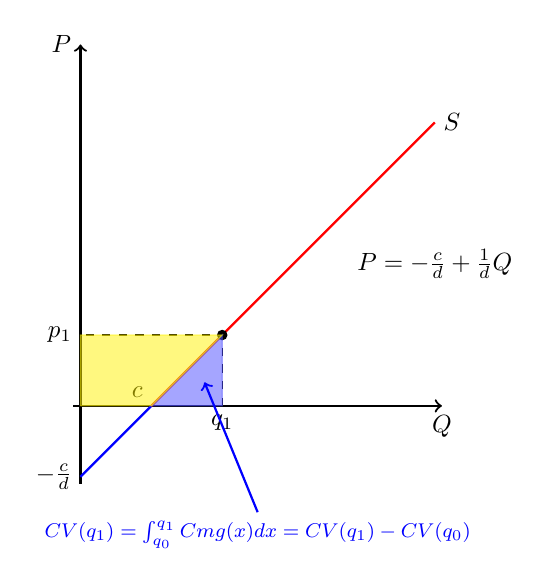
\begin{tikzpicture}[
					scale = .9,
					every node/.style = {scale = .9},
					declare function = {
						s(\x) = -(1/1)+(1/1)*\x;
					}]

					\draw[->,thick] (-0.1,-0) -- (5.1,-0) node[below]{$Q$};
					\draw[->,thick] (0,-1.1) -- (0,5.1) node[left]{$P$};

					\draw[blue,thick,domain=0:1,variable=\x] plot (\x,{s(\x)});
					\draw[red,thick,domain=1:5,variable=\x] plot (\x,{s(\x)});
					
					\draw(0,{s(0)}) node[left]{\(-\frac{c}{d}\)};
					\draw(1,{s(1)}) node[above left] {$c$};

					\draw(5,{s(5)}) node[right]{$S$};

					\draw(5,{s(5)/2}) node[]{\(P=-\frac{c}{d}+\frac{1}{d}Q\)};

					\draw[dashed](2,0) node[below]{$q_1$} -- (2,{s(2)})node[circle,fill,inner sep=1.5]{} -- (0,{s(2)})node[left]{$p_1$};

					\onslide<2->{
						\draw[fill,blue!70!white,opacity=0.5] (1,0) -- (2,0) -- (2,{s(2)}) -- (1,0);
						\draw[<-,blue,thick] (1.75,{s(2)/3}) -- (2.5,{-s(2)-0.5})node[below]{\footnotesize\(CV(q_1)=\int^{q_1}_{q_0}Cmg(x)dx=CV(q_1)-CV(q_0)\)};
					}

					\onslide<3->{
						\draw[fill,yellow,opacity=0.5] (0,0) -- (1,0) -- (2,{s(2)}) -- (0,{s(2)}) -- (0,0);
					}

				\end{tikzpicture}
			\end{center}
		\end{column}
		\begin{column}{0.4\textwidth}
			{
			\small
			\begin{itemize}
				\item Para produzir $q_1$, no minimo os produtores t\^em de receber $p_1$ por unidade, ou, ao pre\c co $p_1$ o m\'aximo que os produtores est\~ao dispostos a produzir \'e $q_1$
				\item $p_1\times q_1$ \'e a receita de vendas; a \'area do triangulo abaixo da Oferta at\'e $q_1$ s\~ao os custos vari\'aveis... a diferen\c ca entre receita e custos vari\'aveis \'e o {\colorbox{yellow}{\textbf{Excedente de Produtor!}}}
			\end{itemize}
			\normalsize
			}
		\end{column}
	\end{columns}
\end{frame}

\begin{frame}
	\frametitle{Excedente do Produtor}
	Por unidade do bem transaccionado, \'e a diferen\c ca entre o que o produtor recebe por unidade e o m\'inimo que estaria disposto a receber para produzir e fornecer essa unidade (valor dado pela curva de oferta)
	
	\vspace{0.5cm}

	O excedente total do produtor \'e o somat\'orio dos excedentes individuais de cada produtor e corresponde graficamente \`a \'area acima da curva de oferta at\'e ao pre\c co.

	\vspace{0.5cm}

	Para empresas economicamente vi\'aveis, o excedente \'e necessariamente n\~ao negativo, o que pode consistir em lucro ou preju\'izo a curto prazo, consoante o n\'ivel de custos fixos.
\end{frame}

\begin{frame}
	\frametitle{Excedente do Produtor}

	\[\text{Lucro}=RT-CV-CF\] 

	\vspace{1cm}

	\[\text{Lucro} = \text{Excedente de produtor} - CF\]

	\vspace{1cm}

	Exerc\'icios recomendados: Caderno 3 $\rightarrow$ 8, 9, 10 e 12.
\end{frame}
\section{Equilibrio de Mercado - Curto Prazo}
\begin{frame}
	\frametitle{Custo M\'edio e Lucro}
	Em geral:
	\begin{align*}
		\text{Lucro} &= \text{Receita Total} - \text{Custo Total}\\
		\Pi &= RT - CT \\
		\Pi &= PQ-CF-CV \\
		\Pi &= Q(P-CTM) = Q(P-CVM-CFM)
	\end{align*}

	Se o pre\c co unit\'ario de venda do bem for suficientemente grande, $P>CTM$, a empresa ter\'a lucro, caso contr\'ario, ter\'a prejuizo.
\end{frame}

\begin{frame}
	\frametitle{Equil\'ibrio no Mercado Competitivo (curto prazo)}
	\begin{itemize}
		\item O mercado est\'a em equil\'ibrio quando se atinge um pre\c co e uma quantidade tais que os consumidores e os produtores n\~ao querem alterar as suas escolhas individuais...\pause
		\item Os consumidores compram exactamente a quantidade que estavam dispostos a adquirir\pause
		\item Os produtores vendem exactamente a quantidade que planificavam oferecer\pause
		\item Ao pre\c co de equil\'ibrio, a quantidade procurada \'e igual \`a quantidade oferecida
	\end{itemize}
\end{frame}

\begin{frame}
	\frametitle{Equil\'ibrio de Mercado}
	\begin{center}
		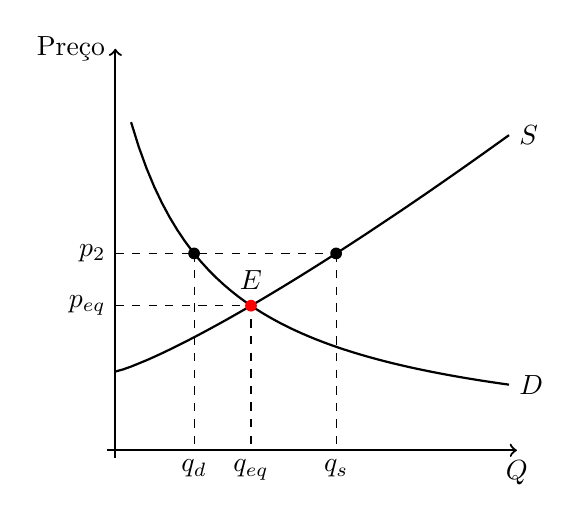
\begin{tikzpicture}[
			scale = 1,
			every node/.style = {scale = 1},
			declare function = {
				s(\x) = 1+(\x/2)^(3/2.5);
				d(\x) = 5/(\x+1);
			}
			]

			\draw[thick,->] (-0.1,0) -- (5.1,0)node[below]{$Q$};
			\draw[thick,->] (0,-0.1) -- (0,5.1)node[left]{Pre\c co};

			\onslide<2->{
				\draw[thick,samples=50,domain=0.2:5,variable=\x] plot (\x,{d(\x)})node[right]{$D$};
			}

			\onslide<3->{
				\draw[thick,samples=50,domain=0:5,variable=\x] plot (\x,{s(\x)})node[right]{$S$};
			}
				
			\def\ea{1}
			\def\eb{2.80397}
			\def\eq{1.72301}

			\onslide<4>{
				\draw(\ea,{d(\ea)}) node[circle,fill,inner sep=1.5]{};
			}

			\only<4>{
				\draw(\eb,{s(\eb)}) node[circle,fill,inner sep=1.5]{};
				\draw[dashed](0,{s(\eb)})node[left]{$p_2$} -- (\eb,{s(\eb)});
				\draw[dashed](\ea,{d(\ea)}) -- (\ea,0)node[below]{$q_d$};
				\draw[dashed](\eb,{s(\eb)}) -- (\eb,0)node[below]{$q_s$};
			}

			\onslide<5->{
				\draw[dashed] (0,{d(\eq)})node[left]{$p_{eq}$} -- (\eq,{d(\eq)}) -- (\eq,0)node[below]{$q_{eq}$};
				\draw(\eq,{d(\eq)}) node[black,circle,fill=red,inner sep=1.5,label=above:{$E$}]{};
			}
			
		\end{tikzpicture}
	\end{center}
\end{frame}

\begin{frame}
	\frametitle{Equil\'ibrio de Mercado}
	\begin{itemize}
		\item O equil\'ibrio surge pelo ajustamento autom\'atico de pre\c co, processo que Adam Smith (1776) baptizou como ``A M\~ao Invis\'ivel,'' desde que os agentes econ\'omicos sejam racionais e, portanto, escolham de forma \'optima
		\item Nos mercados concorrenciais, n\~ao havendo falhas de mercado, este equil\'ibrio \'e eficiente!
	\end{itemize}
\end{frame}

\begin{frame}
	\frametitle{Excesso de Oferta: o pre\c co desce}
	\begin{center}
		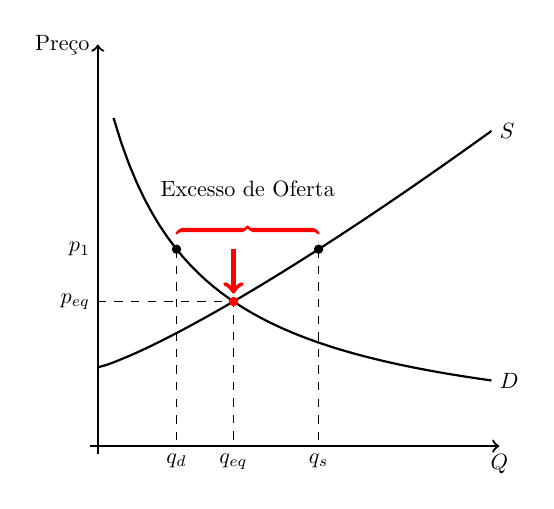
\begin{tikzpicture}[
			scale = 1,
			every node/.style = {scale = 0.8},
			declare function = {
				s(\x) = 1+(\x/2)^(3/2.5);
				d(\x) = 5/(\x+1);
			}
			]

			\draw[thick,->] (-0.1,0) -- (5.1,0)node[below]{$Q$};
			\draw[thick,->] (0,-0.1) -- (0,5.1)node[left]{Pre\c co};

			\draw[thick,samples=50,domain=0.2:5,variable=\x] plot (\x,{d(\x)})node[right]{$D$};
			\draw[thick,samples=50,domain=0:5,variable=\x] plot (\x,{s(\x)})node[right]{$S$};
				
			\def\ea{1}
			\def\eb{2.80397}
			\def\eq{1.72301}

			\draw(\ea,{d(\ea)}) node[circle,fill,inner sep=1.5]{};

			\draw(\eb,{s(\eb)}) node[circle,fill,inner sep=1.5]{};
			\draw[draw=none](0,{s(\eb)})node[left]{$p_1$} -- (\eb,{s(\eb)});
			\draw[dashed](\ea,{d(\ea)}) -- (\ea,0)node[below]{$q_d$};
			\draw[dashed](\eb,{s(\eb)}) -- (\eb,0)node[below]{$q_s$};

			\draw[dashed] (0,{d(\eq)})node[left]{$p_{eq}$} -- (\eq,{d(\eq)}) -- (\eq,0)node[below]{$q_{eq}$};
			\draw[pen colour={red},ultra thick,decorate,decoration={calligraphic brace},yshift=0.2cm] (\ea,{d(\ea)}) -- (\eb,{s(\eb)}) node[midway,above=10pt]{Excesso de Oferta};

			\draw(\eq,{d(\eq)}) node[black,circle,fill=red,inner sep=1.5]{};

			\onslide<2>{
				\draw[ultra thick, red, ->] (\eq,{d(\ea)}) -- (\eq,{d(\eq)+0.1});
			}
			
		\end{tikzpicture}
	\end{center}
	\[p=p_1 \ \Rightarrow \ q_s>q_d\]
\end{frame}

\begin{frame}
	\frametitle{Excesso de Procura: o pre\c co sobe}
	\begin{center}
		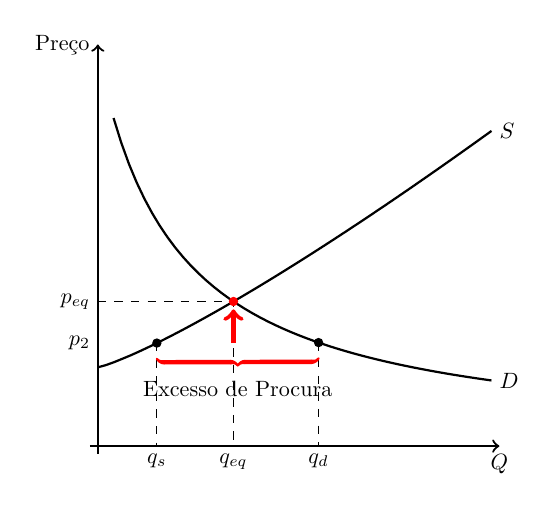
\begin{tikzpicture}[
			scale = 1,
			every node/.style = {scale = 0.8},
			declare function = {
				s(\x) = 1+(\x/2)^(3/2.5);
				d(\x) = 5/(\x+1);
			}
			]

			\draw[thick,->] (-0.1,0) -- (5.1,0)node[below]{$Q$};
			\draw[thick,->] (0,-0.1) -- (0,5.1)node[left]{Pre\c co};

			\draw[thick,samples=50,domain=0.2:5,variable=\x] plot (\x,{d(\x)})node[right]{$D$};
			\draw[thick,samples=50,domain=0:5,variable=\x] plot (\x,{s(\x)})node[right]{$S$};
				
			\def\ea{0.75}
			\def\eb{2.80397}
			\def\eq{1.72301}

			\draw(\ea,{s(\ea)}) node[circle,fill,inner sep=1.5]{};

			\draw(\eb,{d(\eb)}) node[circle,fill,inner sep=1.5]{};
			\draw[draw=none](0,{s(\ea)})node[left]{$p_2$} -- (\eb,{d(\eb)});
			\draw[dashed](\ea,{s(\ea)}) -- (\ea,0)node[below]{$q_s$};
			\draw[dashed](\eb,{d(\eb)}) -- (\eb,0)node[below]{$q_d$};

			\draw[dashed] (0,{d(\eq)})node[left]{$p_{eq}$} -- (\eq,{d(\eq)}) -- (\eq,0)node[below]{$q_{eq}$};
			\draw[pen colour={red},ultra thick,decorate,decoration={calligraphic brace,mirror},yshift=-0.2cm] (\ea,{s(\ea)}) -- (\eb,{d(\eb)}) node[midway,below=5pt]{Excesso de Procura};

			\draw(\eq,{s(\eq)}) node[black,circle,fill=red,inner sep=1.5]{};

			\onslide<2>{
				\draw[ultra thick, red, ->] (\eq,{s(\ea)}) -- (\eq,{s(\eq)-0.1});
			}
			
		\end{tikzpicture}
	\end{center}
	\[p=p_2 \ \Rightarrow \ q_s<q_d\]
\end{frame}

\begin{frame}
	\frametitle{Altera\c c\~oes ao Equil\'ibrio: Expans\~ao de Procura}
	\begin{center}
		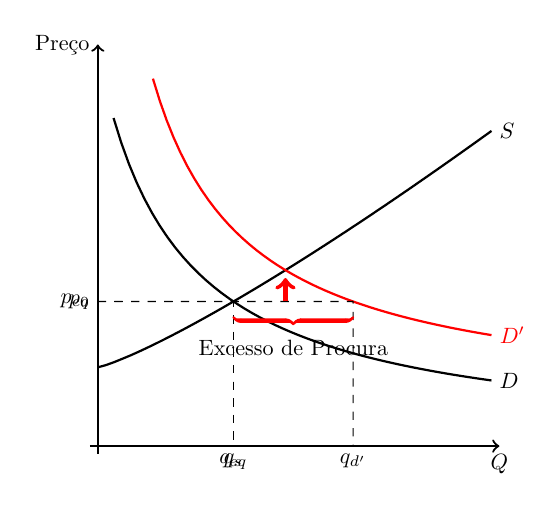
\begin{tikzpicture}[
			scale = 1,
			every node/.style = {scale = 0.8},
			declare function = {
				s(\x) = 1+(\x/2)^(3/2.5);
				d(\x) = 5/(\x+1);
				d2(\x) = d(\x-0.5)+0.5;
			}
			]

			\def\ea{0.75}
			\def\eb{2.80397}
			\def\eq{1.72301}
			\def\noeq{3.2419455}
			\def\neweq{2.38325}

			\draw[thick,->] (-0.1,0) -- (5.1,0)node[below]{$Q$};
			\draw[thick,->] (0,-0.1) -- (0,5.1)node[left]{Pre\c co};

			\draw[thick,samples=50,domain=0:5,variable=\x] plot (\x,{s(\x)})node[right]{$S$};

			\onslide<1-2>{
				\draw[dashed] (0,{d(\eq)})node[left]{$p_{eq}$} -- (\eq,{d(\eq)}) -- (\eq,0)node[below]{$q_{eq}$};
			}

			\onslide<1-3>{
				\draw[thick,samples=50,domain=0.2:5,variable=\x] plot (\x,{d(\x)})node[right]{$D$};
			}

			\onslide<2->{
				\draw[thick,red,samples=50,domain=0.7:5,variable=\x] plot (\x,{d2(\x)})node[right]{$D'$};
			}

			\onslide<3->{
				\draw[dashed] (0,{d(\eq)})node[left]{$p_{0}$} -- (\eq,{d(\eq)}) -- (\eq,0)node[below]{$q_{s}$};
				\draw[dashed] (0,{d(\eq)}) -- (\noeq,{d2(\noeq)}) -- (\noeq,0)node[below]{$q_{d'}$};
			}

			\onslide<4->{
				\draw[pen colour={red},ultra thick,decorate,decoration={calligraphic brace,mirror},yshift=-0.2cm] (\eq,{s(\eq)}) -- (\noeq,{d2(\noeq)}) node[midway,below=5pt]{Excesso de Procura};
			}
			
			\onslide<5>{
				\draw[ultra thick, red, ->] (\neweq,{s(\eq)}) -- (\neweq,{s(\neweq)-0.1});
			}

		\end{tikzpicture}
	\end{center}
\end{frame}

\begin{frame}
	\frametitle{Altera\c c\~oes ao Equil\'ibrio: Expans\~ao de Oferta}
	\begin{center}
		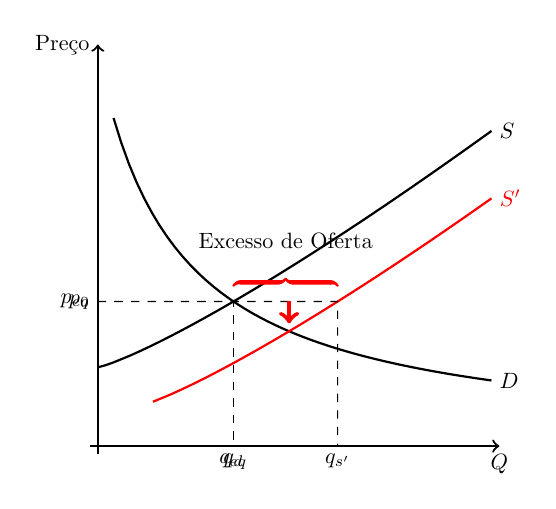
\begin{tikzpicture}[
			scale = 1,
			every node/.style = {scale = 0.8},
			declare function = {
				s(\x) = 1+(\x/2)^(3/2.5);
				s2(\x) = s(\x-0.5)-0.5;
				d(\x) = 5/(\x+1);
				d2(\x) = d(\x-0.5)+0.5;
			}
			]

			\def\ea{0.75}
			\def\eb{2.80397}
			\def\eq{1.72301}
			\def\noeq{3.04638}
			\def\neweq{2.42959}

			\draw[thick,->] (-0.1,0) -- (5.1,0)node[below]{$Q$};
			\draw[thick,->] (0,-0.1) -- (0,5.1)node[left]{Pre\c co};

			\draw[thick,samples=50,domain=0.2:5,variable=\x] plot (\x,{d(\x)})node[right]{$D$};;

			\onslide<1-2>{
				\draw[dashed] (0,{d(\eq)})node[left]{$p_{eq}$} -- (\eq,{d(\eq)}) -- (\eq,0)node[below]{$q_{eq}$};
			}

			\onslide<1-3>{
				\draw[thick,samples=50,domain=0:5,variable=\x] plot (\x,{s(\x)})node[right]{$S$};
			}

			\onslide<2->{
				\draw[thick,red,samples=50,domain=0.7:5,variable=\x] plot (\x,{s2(\x)})node[right]{$S'$};
			}

			\onslide<3->{
				\draw[dashed] (0,{d(\eq)})node[left]{$p_{0}$} -- (\eq,{d(\eq)}) -- (\eq,0)node[below]{$q_{d}$};
				\draw[dashed] (0,{d(\eq)}) -- (\noeq,{s2(\noeq)}) -- (\noeq,0)node[below]{$q_{s'}$};
			}

			\onslide<4->{
			\draw[pen colour={red},ultra thick,decorate,decoration={calligraphic brace},yshift=0.2cm] (\eq,{d(\eq)}) -- (\noeq,{s2(\noeq)}) node[midway,above=10pt]{Excesso de Oferta};
			}
			
			\onslide<5>{
				\draw[ultra thick, red, ->] (\neweq,{s(\eq)}) -- (\neweq,{s2(\neweq)+0.1});
			}

		\end{tikzpicture}
	\end{center}
\end{frame}

\begin{frame}
	\frametitle{Expans\~ao da Procura/Oferta}
	\begin{center}
		{
		\renewcommand{\arraystretch}{2}
		\begin{tabular}{|c|cc|}
			\hline
			& Q & P \\
			\hline \hline
			$\uparrow$ Procura & $\uparrow$ & $\uparrow$ \\
			$\uparrow$ Oferta & $\uparrow$ & $\downarrow$ \\
			$\uparrow$ Procura e $\uparrow$ Oferta & $\uparrow$ & ? \\
			\hline
		\end{tabular}
		}
	\end{center}
\end{frame}

\begin{frame}
	\frametitle{Altera\c c\~oes ao Equil\'ibrio: Expans\~ao de Oferta}
	\begin{center}
		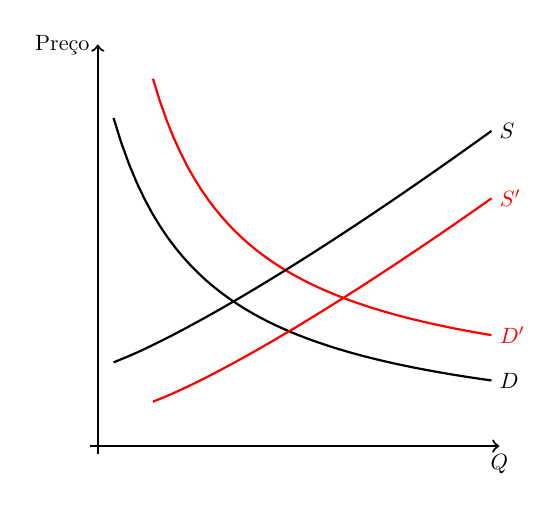
\begin{tikzpicture}[
			scale = 1,
			every node/.style = {scale = 0.8},
			declare function = {
				s(\x) = 1+(\x/2)^(3/2.5);
				s2(\x) = s(\x-0.5)-0.5;
				d(\x) = 5/(\x+1);
				d2(\x) = d(\x-0.5)+0.5;
			}
			]

			\def\ea{0.75}
			\def\eb{2.80397}
			\def\eq{1.72301}
			\def\noeq{3.04638}
			\def\neweq{2.42959}

			\draw[thick,->] (-0.1,0) -- (5.1,0)node[below]{$Q$};
			\draw[thick,->] (0,-0.1) -- (0,5.1)node[left]{Pre\c co};

			\draw[thick,samples=50,domain=0.2:5,variable=\x] plot (\x,{d(\x)})node[right]{$D$};
			\draw[red,thick,samples=50,domain=0.7:5,variable=\x] plot (\x,{d2(\x)})node[right]{$D'$};
			\draw[thick,samples=50,domain=0.2:5,variable=\x] plot (\x,{s(\x)})node[right]{$S$};
			\draw[red,thick,samples=50,domain=0.7:5,variable=\x] plot (\x,{s2(\x)})node[right]{$S'$};

		\end{tikzpicture}
	\end{center}
\end{frame}

\begin{frame}
	\frametitle{Excedente Econ\'omico}
	{\color{green!50!black} Excedente do consumidor} e {\color{blue} Excedente do produtor}
	\begin{columns}
		\begin{column}{0.45\textwidth}
			\begin{center}
				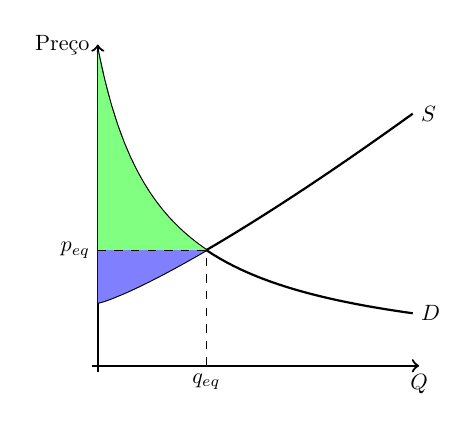
\begin{tikzpicture}[
					scale = 0.8,
					every node/.style = {scale = 0.8},
					declare function = {
						s(\x) = 1+(\x/2)^(3/2.5);
						d(\x) = 5/(\x+1);
					}
					]

					\def\ea{0.75}
					\def\eb{2.80397}
					\def\eq{1.72301}

					\draw[thick,->] (-0.1,0) -- (5.1,0)node[below]{$Q$};
					\draw[thick,->] (0,-0.1) -- (0,5.1)node[left]{Pre\c co};

					\draw[thick,samples=50,domain=0:5,variable=\x] plot (\x,{d(\x)}) node[right]{$D$};
					\draw[thick,samples=50,domain=0:5,variable=\x] plot (\x,{s(\x)}) node[right]{$S$};
					
					\fill[green!50!white,domain=0:\eq,variable=\x] plot (\x,{d(\x)}) -- (0,{d(\eq)});
					\fill[blue!50!white,domain=0:\eq,variable=\x] plot (\x,{s(\x)}) -- (0,{s(\eq)});

					\draw[dashed] (0,{s(\eq)})node[left]{$p_{eq}$} -- (\eq,{s(\eq)}) -- (\eq,0)node[below]{$q_{eq}$};

				\end{tikzpicture}
			\end{center}
		\end{column}
		\begin{column}{0.45\textwidth}
			\begin{center}
				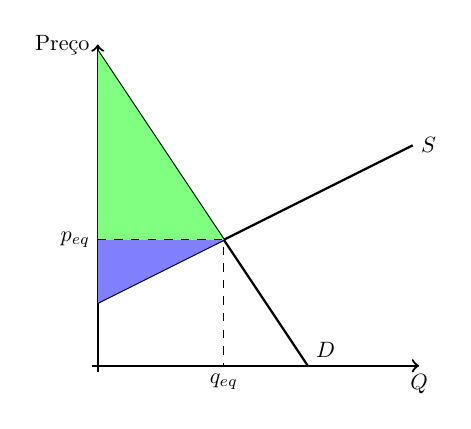
\begin{tikzpicture}[
					scale = 0.8,
					every node/.style = {scale = 0.8},
					declare function = {
						s(\x) = 1+(\x/2);
						d(\x) = 5-(3/2)*\x;
					}
					]

					\def\eq{2}

					\draw[thick,->] (-0.1,0) -- (5.1,0)node[below]{$Q$};
					\draw[thick,->] (0,-0.1) -- (0,5.1)node[left]{Pre\c co};

					\draw[thick,domain=0:(10/3),variable=\x] plot (\x,{d(\x)}) node[above right]{$D$};
					\draw[thick,domain=0:5,variable=\x] plot (\x,{s(\x)}) node[right]{$S$};

					\fill[green!50!white,domain=0:\eq,variable=\x] plot(\x,{d(\x)}) -- (0,{d(\eq)});
					\fill[blue!50!white,domain=0:\eq,variable=\x] plot(\x,{s(\x)}) -- (0,{s(\eq)});

					\draw[dashed] (0,{s(\eq)})node[left]{$p_{eq}$} -- (\eq,{s(\eq)}) -- (\eq,0)node[below]{$q_{eq}$};

				\end{tikzpicture}
			\end{center}
		\end{column}
	\end{columns}
	{\raggedleft{Na vers\~ao linear para o mercado.\par}}
\end{frame}

\begin{frame}
	\frametitle{Excedente Econ\'omico}
	\begin{itemize}
		\setlength\itemsep{1em}
		\item O Excedente Econ\'omico \'e o somat\'orio do excedente do consumidor e do excedente do produtor e representa o valor da exist\^encia de trocas no mercado. Avalia-se nas unidades monet\'arias em que est\~ao expressos os pre\c cos.
		\item Demonstra-se que este excedente \'e m\'aximo num mercado de concorr\^encia perfeita, da\'i se designar como a forma eficiente de mercado (desde que n\~ao existam falhas de mercado)
	\end{itemize}
\end{frame}

\begin{frame}
	\frametitle{Concorr\^encia Perfeita: Escolha indiv. vs Eq. de Mercado}
	A escolha \'optima de produ\c c\~ao, para cada empresa $i$, dar-se-\'a ao longo da curva de procura que lhe \'e dirigida, $D_i$, ao n\'ivel do pre\c co de equil\'ibrio $p^*$, formado pela interac\c c\~ao do conjunto dos agentes econ\'omicos.
	\begin{center}
		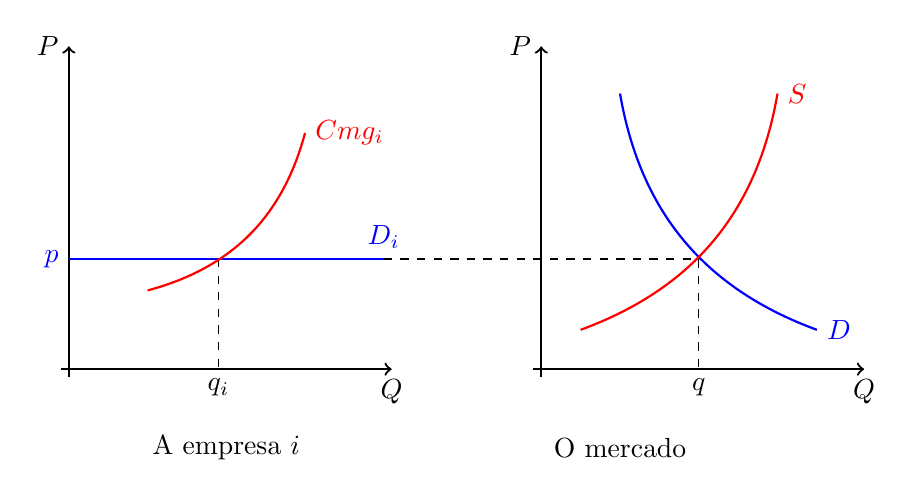
\begin{tikzpicture}[
			scale = 1,
			every node/.style = {scale = 1}
			]

			\def\p{1.4}
			\def\q{8}
			\def\qi{1.9}
			

			\draw[thick,->] (-0.1,0) -- (4.1,0) node[below]{$Q$};
			\draw[thick,->] (5.9,0) -- (10.1,0) node[below]{$Q$};

			\draw[thick,->] (0,-0.1) -- (0,4.1) node[left]{$P$};
			\draw[thick,->] (6,-0.1) -- (6,4.1) node[left]{$P$};

			\draw[thick,blue] (0,\p)node[left]{$p$} -- (4,\p)node[above]{$D_i$};
			\draw[dashed] (\qi,\p) -- (\qi,0)node[below]{$q_i$};
			\draw[dashed] (4,\p) -- (\q,\p) -- (\q,0)node[below]{$q$};

			\draw[red,thick] (1,1) to [bend right] (3,3) node[right]{$Cmg_i$};

			\draw[blue,thick] (7,3.5) to [bend right] (9.5,0.5)node[right]{$D$};
			\draw[red,thick] (6.5,0.5) to [bend right] (9,3.5)node[right]{$S$};

			\draw(2,-1) node {A empresa $i$};
			\draw(7,-1) node {O mercado};

		\end{tikzpicture}
	\end{center}
	
\end{frame}
\section{Equilibrio de Mercado - Longo Prazo}
\begin{frame}
	\frametitle{Longo Prazo}
	\begin{itemize}
		\setlength\itemsep{1em}
		\item Ao longo prazo todos os factores produtivos se alteram e, assim, n\~ao existem custos fixos.
		\item A empresa tem mais alternativas e pode tomar decis\~oes que lhe estavam vedadas no curto prazo.
	\end{itemize}
\end{frame}

\begin{frame}
	\frametitle{Problema da empresa a longo prazo}
		Determinar a melhor combina\c c\~ao de $K$ e $L$ que permitem obter dada produ\c c\~ao ($Q^*$) ao menor custo: 
		\begin{align*}
			Min_{K,L}\ &rK+wL\\
			 s.a.\ &F(K,L)=Q^*
		\end{align*}
\end{frame}

\begin{frame}
	\frametitle{$F(K,L)=Q^*$}
	\begin{itemize}
		\setlength\itemsep{1em}
		\item A condi\c c\~ao $F(K,L)=Q^*$ representa todas as combina\c c\~oes de $K$ e $L$ que permitem atingir a mesma quantidade produzida. Definem uma \textbf{isoquanta}, isto \'e, uma curva de n\'ivel da fun\c c\~ao $F(K,L)$ ao n\'ivel de $Q^*$.
		\item Graficamente, para fun\c c\~oes de produ\c c\~ao da fam\'ilia $F(K,L)=AK^aL^b$ uma isoquanta \'e uma hip\'erbole no espa\c co ($K,L$).
	\end{itemize}
\end{frame}

\begin{frame}
	\frametitle{$F(K,L)=Q^*$}
	\begin{center}
		\begin{tikzpicture}[
			scale = 1,
			every node/.style = {scale = 1}
			]

			\draw[thick,->] (-0.1,0) -- (5.1,0)node[below]{$L$};
			\draw[thick,->] (0,-0.1) -- (0,5.1)node[left]{$K$};

			\draw (0.5,3.5) to [bend right] (3,0.5)node[right]{$Q^*$};
			\draw (1,4) to [bend right] (3.5,1)node[right]{$Q^{**}$};
			\draw (1.5,4.5) to [bend right] (4,1.5)node[right]{$Q^{***}$};

		\end{tikzpicture}
	\end{center}
\end{frame}

\begin{frame}
	\frametitle{Exemplo}
	Se a fun\c c\~ao de produ\c c\~ao for \[Q=K^{0.5}L^{0.5}\]

	No espa\c co $(L,K)$ todas as combina\c c\~oes de capital e trabalho que permitem atingir a produ\c c\~ao $Q=100$ podem ser representadas pela \emph{\textbf{isoquanta}} de equa\c c\~ao:\[100=K^{0.5}L^{0.5}\] ou seja $L=\frac{10,000}{K}$
\end{frame}

\begin{frame}
	\frametitle{Exemplo}
	Ent\~ao para obter a produ\c c\~ao $Q=100$ de forma a minimizar custos ($K$ e $L$) qual a melhor combina\c c\~ao de factores? Se admitirmos que cada factor \'e remunerado a 5um por unidade, o problema do produtor ser\'a 
	\begin{align*}
		\min_{K,L} \ 5K+5L\\
		s.a. \ 100=K^{0.5}L^{0.5}
	\end{align*}

	Proceder por substitui\c c\~ao, da restri\c c\~ao obtemos $K$, ou $L$, reemplazamos na fun\c c\~ao a optimizar, e resolvemos agora s\'o com uma vari\'avel!

\end{frame}

\begin{frame}
	\frametitle{Exemplo}
	Por substitui\c c\~ao de vari\'avel, \'e f\'acil obter: \(L=\frac{10,000}{K}\), e logo \[CT(K)=5K+5\times\frac{10,000}{K}\]
	O m\'inimo de $CT$ em $K$ obter-se-\'a com a derivada em zero (CPO):
	\begin{align*}
		\frac{\partial CT}{\partial K}=5-\frac{50,000}{K^2}=0 \ \Rightarrow \ K^2 = 10,000 \ \Rightarrow \ K = 100
	\end{align*}
	Logo $L=100$, e $CT=1,000$ no \'optimo.
\end{frame}

\begin{frame}
	\frametitle{Isocusto}

	\begin{tcolorbox}[title=\textbf{Isocusto},colback=iscal_color!20!white,colframe=iscal_color]
		Recta formada por todas as combina\c c\~oes de $K$ e $L$ que t\^em o mesmo custo total: \[\overline{CT}=r\times K + w\times L\]
	\end{tcolorbox}

	No exemplo, essa recta tem equa\c c\~ao $1,000=5K+5L$

	\vspace{0.5cm}

	Graficamente, tangencia a \textbf{Isoquanta} $L=\frac{10,000}{K}$ no ponto \'optimo $K=100$, $L=100$

\end{frame}

\begin{frame}
	\frametitle{\(100 = K^{0.5}L^{0.5}\) \\  \(1,000 = 5K+5L\)}
	\begin{center}
		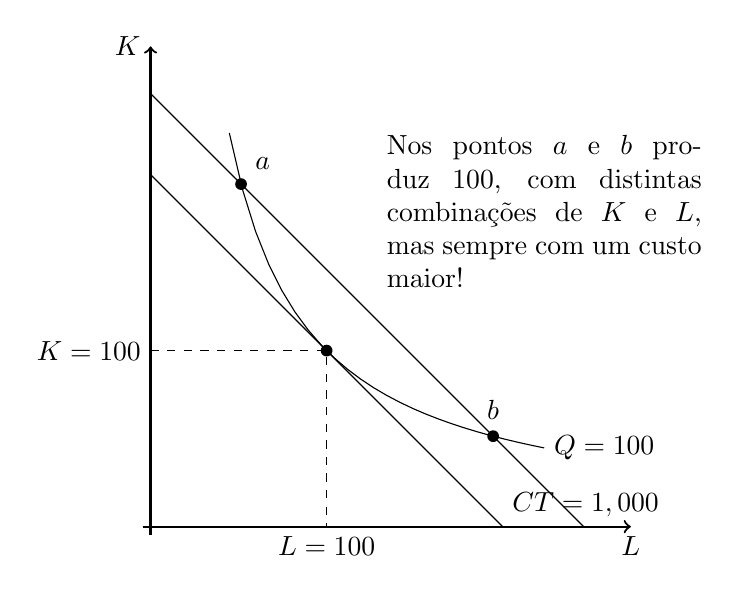
\begin{tikzpicture}[
			scale = 1,
			every node/.style = {scale = 1},
			declare function = {
				iq(\x) = 5/\x;
				ic(\a,\x) = \a-\x;
			}
			]

			\def\w{4.472}
			\def\ww{5.5}
			\def\eq{2.236}

			\draw[thick,->] (-0.1,0) -- (6.1,0)node[below]{$L$};
			\draw[thick,->] (0,-0.1) -- (0,6.1)node[left]{$K$};

			\onslide<2->{
				\draw [domain=1:5,variable=\x] plot (\x,{iq(\x)})node[right]{$Q=100$};
				\draw [domain=0:\w,variable=\x] plot (\x,{ic(\w,\x)});
			}

			\onslide<2-3>{
				\draw(\w,{ic(\w,\w)})node[above right]{$CT=1,000$};
			}

			\onslide<3->{
				\draw[dashed](0,{iq(\eq)})node[left]{$K=100$} -- (\eq,{iq(\eq)}) node[circle,fill,inner sep=1.5 pt]{} -- (\eq,0)node[below]{$L=100$};
			}

			\def\la{1.1492}
			\def\lb{4.3508}

			\onslide<4->{
				\draw [domain=0:\ww,variable=\x] plot (\x,{ic(\ww,\x)});
				\draw (\la,{ic(\ww,\la)})node[circle,fill,inner sep=1.5pt,label=above right:{$a$}]{};
				\draw (\lb,{ic(\ww,\lb)})node[circle,fill,inner sep=1.5pt,label=above:{$b$}]{};
				\draw (5,4)node{\parbox{4cm}{Nos pontos $a$ e $b$ produz 100, com distintas combina\c c\~oes de $K$ e $L$, mas sempre com um custo maior!}};
			}



		\end{tikzpicture}
	\end{center}
\end{frame}

\begin{frame}
	\frametitle{Os custos de longo prazo s\~ao menores}
	\begin{center}
		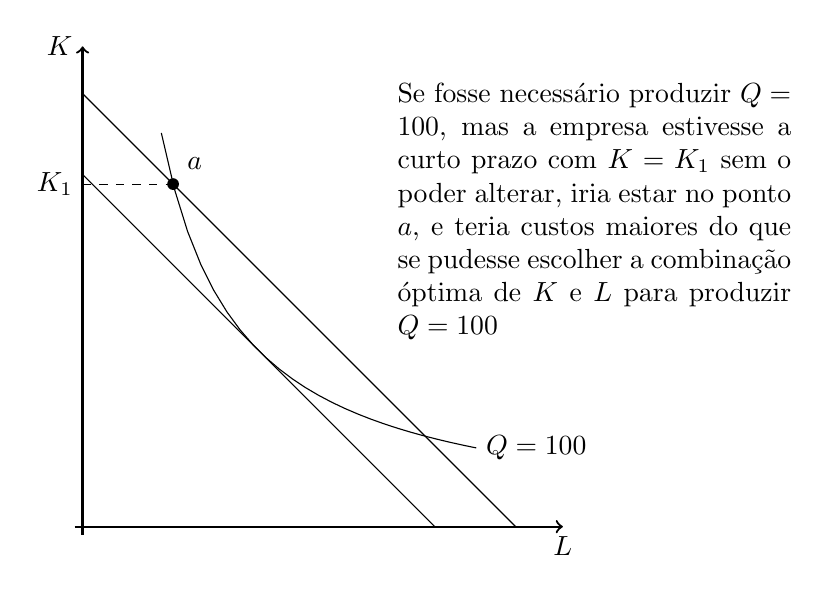
\begin{tikzpicture}[
			scale = 1,
			every node/.style = {scale = 1},
			declare function = {
				iq(\x) = 5/\x;
				ic(\a,\x) = \a-\x;
			}
			]

			\def\w{4.472}
			\def\ww{5.5}
			\def\eq{2.236}

			\draw[thick,->] (-0.1,0) -- (6.1,0)node[below]{$L$};
			\draw[thick,->] (0,-0.1) -- (0,6.1)node[left]{$K$};

			\draw [domain=1:5,variable=\x] plot (\x,{iq(\x)})node[right]{$Q=100$};
			\draw [domain=0:\w,variable=\x] plot (\x,{ic(\w,\x)});
			%\draw(\w,{ic(\w,\w)})node[above right]{$CT=1,000$};
			%\draw[dashed](0,{iq(\eq)})node[left]{$K=100$} -- (\eq,{iq(\eq)}) node[circle,fill,inner sep=1.5 pt]{} -- (\eq,0)node[below]{$L=100$};

			\def\la{1.1492}
			\def\lb{4.3508}

			\draw [domain=0:\ww,variable=\x] plot (\x,{ic(\ww,\x)});
			\draw (\la,{ic(\ww,\la)})node[circle,fill,inner sep=1.5pt,label=above right:{$a$}]{};
			%\draw (\lb,{ic(\ww,\lb)})node[circle,fill,inner sep=1.5pt,label=above:{$b$}]{};
			\draw (6.5,4)node{\parbox{5cm}{Se fosse necess\'ario produzir $Q=100$, mas a empresa estivesse a curto prazo com $K=K_1$ sem o poder alterar, iria estar no ponto $a$, e teria custos maiores do que se pudesse escolher a combina\c c\~ao \'optima de $K$ e $L$ para produzir $Q=100$}};

			\draw[dashed](0,{ic(\ww,\la)})node[left]{$K_1$} -- (\la,{ic(\ww,\la)});

		\end{tikzpicture}
	\end{center}
\end{frame}


\begin{frame}
	\frametitle{Custos de longo prazo}
	\begin{itemize}
		\setlength\itemsep{1em}
		\item A longo prazo, a empresa escolhe as quantidades economicamente eficientes de trabalho e capital que minimizam o custo da produ\c c\~ao de uma dada quantidade a colocar no mercado, que por sua vez depende das exig\^encias do mercado impostas pela procura e pela concorr\^encia que a empresa enfrenta
		\item \textbf{...ent\~ao, a longo prazo os custos m\'edios ser\~ao sempre menores ou iguais aos custos de curto prazo}
	\end{itemize}
\end{frame}

\begin{frame}
	\frametitle{Custos m\'edios a longo prazo}
	\begin{center}
		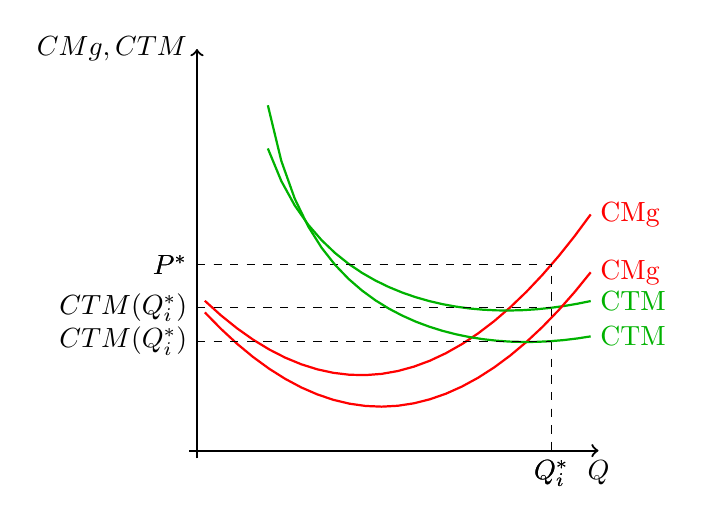
\begin{tikzpicture}[
			scale = 1,
			every node/.style = {scale = 1},
			declare function = {
				cv(\x) = \x - (1/4)*\x^2 + (1/25)*\x^3;
				cf(\x) = 1;
				ct(\x) = cv(\x) + cf(\x);
				cmg(\x) = 1 - (2/4)*\x + (3/25)*\x^2;
				ctm(\x) = ct(\x)/\x;
				cmg2(\x) = 0.8 - (2/4)*(\x-0.25) + (3/25)*(\x-0.25)^2;
				ctm2(\x) = ct(\x-0.25)/(\x-0.25)-0.2;
				cvm(\x) = cv(\x)/\x;
			}]

			\def\p{4.5}

			\draw[->,thick] (-0.1,-0) -- (5.1,-0) node[below]{$Q$};
			\draw[->,thick] (0,-0.1) -- (0,5.1) node[left]{$CMg,CTM$};

			\onslide<1>{

				\draw[red,thick,domain=0.1:5,variable=\x] plot (\x,{2*cmg(\x)-0});
				\draw[red](5,{2*cmg(5)-0})node[right]{CMg};

				\draw[dashed] (0,{2*cmg(\p)})node[left]{$P^*$} -- (\p,{2*cmg(\p)}) -- (\p,0)node[below]{$Q_i^*$};		

				\draw[green!70!black,thick,domain=0.9:5,variable=\x] plot (\x,{2*ctm(\x)-0});
				\draw[green!70!black](5,{2*ctm(5)-0})node[right]{CTM};

				\draw[dashed] (0,{2*ctm(\p)})node[left]{$CTM(Q_i^*)$} -- (\p,{2*ctm(\p)});

			}

			\onslide<2>{

				\draw[opacity=0.2,red,domain=0.1:5,variable=\x] plot (\x,{2*cmg(\x)-0});
				\draw[opacity=0.2,red](5,{2*cmg(5)-0})node[right]{CMg};

				\draw[dashed] (0,{2*cmg(\p)})node[left]{$P^*$} -- (\p,{2*cmg(\p)}) -- (\p,0)node[below]{$Q_i^*$};		

				\draw[opacity=0.2,green!70!black,domain=0.9:5,variable=\x] plot (\x,{2*ctm(\x)-0});
				\draw[opacity=0.2,green!70!black](5,{2*ctm(5)-0})node[right]{CTM};

				\draw[opacity=0.2,dashed] (0,{2*ctm(\p)})node[left]{$CTM(Q_i^*)$} -- (\p,{2*ctm(\p)});

				%==========================================================================

				\draw[red,thick,domain=0.1:5,variable=\x] plot (\x,{2*cmg2(\x)-0});
				\draw[red](5,{2*cmg2(5)-0})node[right]{CMg};		

				\draw[green!70!black,thick,domain=0.9:5,variable=\x] plot (\x,{2*ctm2(\x)-0});
				\draw[green!70!black](5,{2*ctm2(5)-0})node[right]{CTM};

				\draw[dashed] (0,{2*ctm2(\p)})node[left]{$CTM(Q_i^*)$} -- (\p,{2*ctm2(\p)});

			}

		\end{tikzpicture}
	\end{center}
\end{frame}

\begin{frame}
	\frametitle{Custos m\'edios a longo prazo}
	\begin{center}
		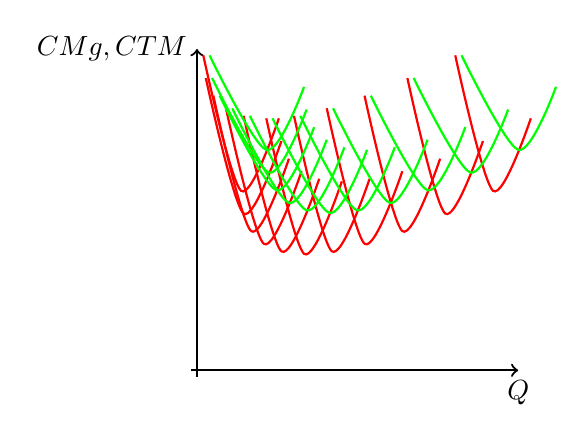
\begin{tikzpicture}[
			scale = 0.8,
			every node/.style = {scale = 1}
			]

			\draw[->,thick] (-0.1,-0) -- (5.1,-0) node[below]{$Q$};
			\draw[->,thick] (0,-0.1) -- (0,5.1) node[left]{$CMg,CTM$};

			\def\con{50}
			\def\conx{50}
			\def\powx{2}
			\def\pow{2}

			\foreach \r in {-50,-40,...,50}{
				\draw[thick,red] plot [smooth] coordinates {
					({0.1+((\r+50)/\conx)^\powx},{4+(\r/\con)^\pow})
					({0.7+((\r+50)/\conx)^\powx},{1.85+(\r/\con)^\pow})
					({1.3+((\r+50)/\conx)^\powx},{3+(\r/\con)^\pow})
					};
			
			}

			\foreach \r in {-50,-40,...,50}{
				\draw[thick,green] plot [smooth] coordinates {
					({0.2+((\r+50)/\conx)^\powx},{4+(\r/\con)^\pow})
					({1.1+((\r+50)/\conx)^\powx},{2.5+(\r/\con)^\pow})
					({1.7+((\r+50)/\conx)^\powx},{3.5+(\r/\con)^\pow})
					};
			}

		\end{tikzpicture}
	\end{center}
\end{frame}

\begin{frame}
	\frametitle{Custos m\'edios a longo prazo}
	\begin{center}
		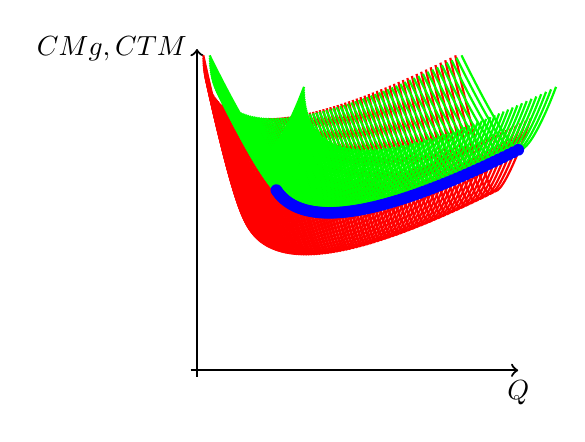
\begin{tikzpicture}[
			scale = 0.8,
			every node/.style = {scale = 1}
			]

			\draw[->,thick] (-0.1,-0) -- (5.1,-0) node[below]{$Q$};
			\draw[->,thick] (0,-0.1) -- (0,5.1) node[left]{$CMg,CTM$};

			\def\con{50}
			\def\conx{50}
			\def\powx{2}
			\def\pow{2}

			\onslide<1-2>{
				\foreach \r in {-50,...,50}{
					\draw[thick,red] plot [smooth] coordinates {
						({0.1+((\r+50)/\conx)^\powx},{4+(\r/\con)^\pow})
						({0.7+((\r+50)/\conx)^\powx},{1.85+(\r/\con)^\pow})
						({1.3+((\r+50)/\conx)^\powx},{3+(\r/\con)^\pow})
						};
				
				}

				\foreach \r in {-50,...,50}{
					\draw[thick,green] plot [smooth] coordinates {
						({0.2+((\r+50)/\conx)^\powx},{4+(\r/\con)^\pow})
						({1.1+((\r+50)/\conx)^\powx},{2.5+(\r/\con)^\pow})
						({1.7+((\r+50)/\conx)^\powx},{3.5+(\r/\con)^\pow})
						};
				}
			}

			\onslide<2-3>{
				\foreach \r in {-30,...,50}{
					\draw({1.1+((\r+50)/\conx)^\powx},{2.5+(\r/\con)^\pow}) node[circle,blue,fill,inner sep=1.5pt]{};
				}
			}

		\end{tikzpicture}
	\end{center}
	\onslide<3>{Curva de Custo M\'edio de Longo Prazo}
\end{frame}

\begin{frame}
	\frametitle{Observa\c c\~ao}
	\begin{itemize}
		\item Os custos aqui referidos s\~ao \textbf{custos econ\'omicos}, ou seja s\~ao \textbf{custos de oportunidade} , que j\'a sabemos inclu\'irem outros valores para al\'em da despesa de quisi\c c\~ao dos fatores de produ\c c\~ao
		\item ent\~ao: um lucro econ\'omico ser\'a sempre n\~ao superior ao lucro contabil\'istico, presente nas Demonstra\c c\~oes de Resultados! Porqu\^e?
		\item Recordar o conceito de Custo de Oportunidade!
	\end{itemize}
\end{frame}

\begin{frame}
	\frametitle{Economias de Escala}
	\begin{itemize}
		\item Enquanto $CM_{LP}$ for decrescente, diz-se que h\'a Economias de Escala
		\item Quando $CM_{LP}$ \'e crescente, diz-se que h\'a Deseconomias de Escala
		\item O m\'inimo de $CM_{LP}$ \'e a Escala M\'inima Eficiente. O n\'ivel de $Q$ onde esse m\'inimo ocorre \'e espec\'ifico \`a tecnologia/sector de atividade.
	\end{itemize}
\end{frame}

\begin{frame}
	\frametitle{Economias de Escala}
	\begin{center}
		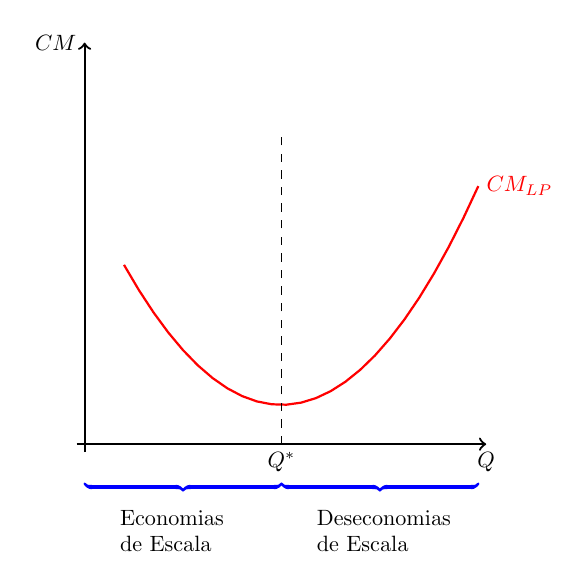
\begin{tikzpicture}[
			scale = 1,
			every node/.style = {scale = 0.8}
			]

			\draw[->,thick] (-0.1,-0) -- (5.1,-0) node[below]{$Q$};
			\draw[->,thick] (0,-0.1) -- (0,5.1) node[left]{$CM$};

			\draw[thick,red,domain=0.5:5,variable=\x] plot (\x,{((\x-2.5)/1.5)^2+0.5})node[right]{$CM_{LP}$};
			\draw[dashed] (2.5,0)node[below]{$Q^*$} -- (2.5,4);

			\draw[pen colour={blue},ultra thick,decorate,decoration={calligraphic brace,mirror},yshift=-0.5cm] (0,0) -- (2.5,0) node[midway,yshift=-0.75cm]{\parbox{2cm}{Economias de Escala}};
			\draw[pen colour={blue},ultra thick,decorate,decoration={calligraphic brace,mirror},yshift=-0.5cm] (2.5,0) -- (5,0) node[midway,yshift=-0.75cm]{\parbox{2cm}{Deseconomias de Escala}};

		\end{tikzpicture}

		Escala M\'inima Eficiente \\ (corresponde a um determinado valor de $K$)
	\end{center}
\end{frame}

\begin{frame}
	\frametitle{Economias de Escala}
	O n\'ivel de $Q$ que minimiza $CM_{LP}$ influencia o n\'umero de empresas (e respectiva dimens\~ao ao n\'ivel de volume de \emph{output}) em cada sector/mercado.

	\vspace{0.5cm}

	Quanto menor a quantidade que minimiza o $CM_{LP}$ maior \'e a tend\^encia para haver mais empresas de menor dimens\~ao, para satisfazer um mercado com uma dada procura

\end{frame}

\begin{frame}
	\frametitle{Concorr\^encia Perfeita (Longo Prazo)}
	Se $\Pi>0$, o mercado \'e atraente: entram mais empresas, expandindo a oferta:
	\begin{center}
		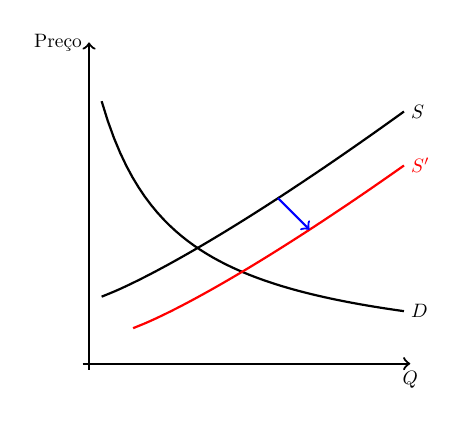
\begin{tikzpicture}[
			scale = 0.8,
			every node/.style = {scale = 0.7},
			declare function = {
				s(\x) = 1+(\x/2)^(3/2.5);
				s2(\x) = s(\x-0.5)-0.5;
				d(\x) = 5/(\x+1);
				d2(\x) = d(\x-0.5)+0.5;
			}
			]

			\def\ea{0.75}
			\def\eb{2.80397}
			\def\eq{1.72301}
			\def\noeq{3.04638}
			\def\neweq{2.42959}

			\draw[thick,->] (-0.1,0) -- (5.1,0)node[below]{$Q$};
			\draw[thick,->] (0,-0.1) -- (0,5.1)node[left]{Pre\c co};

			\draw[thick,samples=50,domain=0.2:5,variable=\x] plot (\x,{d(\x)})node[right]{$D$};
			\draw[thick,samples=50,domain=0.2:5,variable=\x] plot (\x,{s(\x)})node[right]{$S$};
			\draw[red,thick,samples=50,domain=0.7:5,variable=\x] plot (\x,{s2(\x)})node[right]{$S'$};

			\draw[->,blue,thick] (3,{s(3)}) -- (3.5,{s2(3.5)});

		\end{tikzpicture}
	\end{center}
	Baixa o pre\c co de equil\'ibrio, aumenta a quantidade, mas cada empresa produz um pouco menos do que antes, porque h\'a mais empresas no mercado... diminui o lucro individual!
\end{frame}

\begin{frame}
	\frametitle{Entrada de Empresas no Mercado}

	\begin{center}
		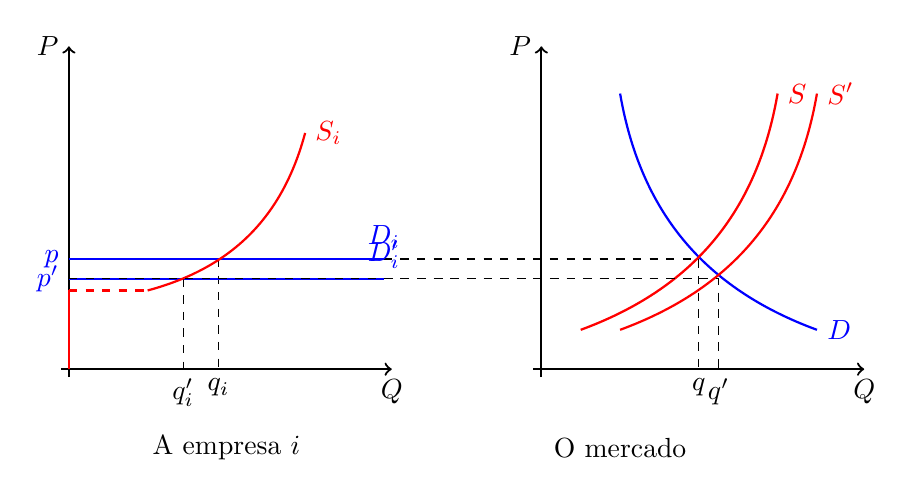
\begin{tikzpicture}[
			scale = 1,
			every node/.style = {scale = 1}
			]

			\def\p{1.4}
			\def\pa{1.15}
			\def\q{8}
			\def\qi{1.9}
			\def\qia{1.45}
			\def\qa{8.25}
			

			\draw[thick,->] (-0.1,0) -- (4.1,0) node[below]{$Q$};
			\draw[thick,->] (5.9,0) -- (10.1,0) node[below]{$Q$};

			\draw[thick,->] (0,-0.1) -- (0,4.1) node[left]{$P$};
			\draw[thick,->] (6,-0.1) -- (6,4.1) node[left]{$P$};

			\onslide<1-3>{
				\draw[thick,blue] (0,\p)node[left]{$p$} -- (4,\p)node[above]{$D_i$};
				\draw[dashed] (\qi,\p) -- (\qi,0)node[below]{$q_i$};
				\draw[dashed] (4,\p) -- (\q,\p) -- (\q,0)node[below]{$q$};
			}

			\onslide<4->{
				\draw[opacity=0.2,thick,blue] (0,\p)node[left]{$p$} -- (4,\p)node[above]{$D_i$};
				\draw[opacity=0.2,dashed] (\qi,\p) -- (\qi,0)node[below]{$q_i$};
				\draw[opacity=0.2,dashed] (4,\p) -- (\q,\p) -- (\q,0)node[below]{$q$};

				\draw[thick,blue] (0,\pa)node[left]{$p'$} -- (4,\pa)node[above]{$D_i'$};
				\draw[dashed] (\qia,\pa) -- (\qia,0)node[below]{$q_i'$};
				\draw[dashed] (4,\pa) -- (\qa,\pa) -- (\qa,0)node[below]{$q'$};
			}

			\draw[red,thick] (1,1) to [bend right] (3,3) node[right]{$S_i$};
			\draw[red,thick] (0,0) -- (0,1);
			\draw[dashed,thick,red] (0,1) -- (1,1);

			\draw[blue,thick] (7,3.5) to [bend right] (9.5,0.5)node[right]{$D$};
			
			\onslide<1-3>{
				\draw[red,thick] (6.5,0.5) to [bend right] (9,3.5)node[right]{$S$};
			}

			\onslide<3->{
				\draw[opacity=0.2,red,thick] (6.5,0.5) to [bend right] (9,3.5)node[right]{$S$};
			}

			\draw(2,-1) node {A empresa $i$};
			\draw(7,-1) node {O mercado};

			\onslide<2->{
				\draw[red,thick] (7,0.5) to [bend right] (9.5,3.5)node[right]{$S'$};				
			}

			\onslide<3->{
				\draw[dashed](0,\pa) -- (\qa,\pa)--(\qa,0);
			}

		\end{tikzpicture}
	\end{center}
	Entram empresas $\rightarrow$ h\'a expans\~ao da oferta $\rightarrow$ pre\c co desce $\rightarrow$ quantidade produzida por cada empresa desce $\rightarrow$ no total, h\'a mais produto no mercado $\rightarrow$ o lucro individual diminui
	
\end{frame}

\begin{frame}
	\frametitle{Equil\'ibrio de Longo Prazo}
	Entrar\~ao empresas no mercado (sair\~ao, caso $\Pi<0$) at\'e que se verifique $\Pi=0$, pelo que o equil\'ibrio de $LP$ \'e tal que: \[p=Cmg_{LP}=CM_{LP}\]
\end{frame}

\begin{frame}
	\frametitle{Equil\'ibrio de Longo Prazo}
	\begin{center}
		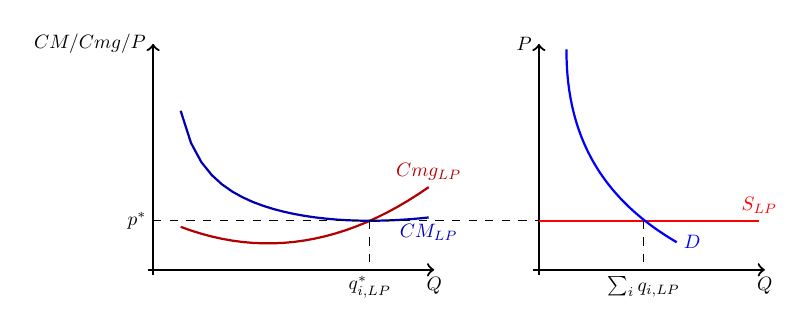
\begin{tikzpicture}[
			scale = 0.7,
			every node/.style = {scale = 0.7},
			declare function = {
				cv(\x) = \x - (1/4)*\x^2 + (1/25)*\x^3;
				cf(\x) = 1;
				ct(\x) = cv(\x) + cf(\x);
				cmg(\x) = 1 - (2/4)*\x + (3/25)*\x^2;
				ctm(\x) = ct(\x)/\x;
				cvm(\x) = cv(\x)/\x;
			}]			

			\def\qs{3.9331}
			\def\qt{8.9}

			\draw[thick,->] (-0.1,0) -- (5.1,0) node[below]{$Q$};
			\draw[thick,->] (6.9,0) -- (11.1,0) node[below]{$Q$};

			\draw[thick,->] (0,-0.1) -- (0,4.1) node[left]{$CM/Cmg/P$};
			\draw[thick,->] (7,-0.1) -- (7,4.1) node[left]{$P$};

			\draw [thick,red!70!black,domain=0.5:5, variable=\x] plot(\x,{cmg(\x)})node[above]{$Cmg_{LP}$};
			\draw [thick,blue!70!black,domain=0.5:5, variable=\x] plot(\x,{ctm(\x)})node[below]{$CM_{LP}$};

			\draw[dashed] (0,{cmg(\qs)})node[left]{$p^*$} -- (7,{cmg(\qs)});
			\draw[dashed] (\qs,{cmg(\qs)}) -- (\qs,0)node[below]{$q^*_{i,LP}$};
			\draw[red,thick] (7,{cmg(\qs)}) -- (11,{cmg(\qs)})node[above]{$S_{LP}$};

			\draw[blue,thick](7.5,4) to [bend right] (9.5,0.5)node[right]{$D$};
			\draw[dashed] (\qt,{cmg(\qs)})--(\qt,0)node[below]{$\sum_{i}q_{i,LP}$};

		\end{tikzpicture}
	\end{center}
	LP: todo o escedente econ\'omico do mercado \'e o Excedente do Consumidor!
\end{frame}

\end{document}